
El razonamiento lógico es lo que ha permitido que la matemática y la ciencia se desarrollen. 
No es nada nuevo en la historia de la humanidad, 
ya los griegos trabajaron en formalizar el razonamiento de manera abstracta, 
distinguiendo entre razonamientos correctos e incorrectos. 

Todas las ciencias usan el razonamiento lógico para avanzar, 
sin embargo en el siglo 
XIX la matemática crea una rama específica para estudiarlo, 
\'esta es la {\em lógica formal}, la cual es muy árida y da lugar 
a importantes teoremas tales como el teorema de G\"odel, del cual 
ya habrán o\'ido hablar.

En este curso no nos vamos a dedicar a la lógica formal, 
sino solo al razonamiento lógico, sin embargo 
nos valdremos de algunas de sus notaciones y criterios 
para así hacer más claros los argumentos que desarrollaremos 
a través del semestre.

\section{Proposiciones lógicas}

El objetivo del razonamiento lógico es descubrir ``verdades''\footnote{Por supuesto el concepto de ``verdad'' es muy complejo y debatido, pero en este curso no tendremos que lidiar con esas dificultades.},
solo se interesa por enunciados afirmativos, susceptibles 
de ser {\em verdaderos} o {\em falsos}, que llamamos 
{\em proposiciones lógicas}.
Del diccionario obtenemos la siguiente definición:

\begin{defn}[Proposición lógica]
Es un enunciado que expresa un concepto que puede ser verdadero o falso.
\end{defn}

\begin{ejemplo}
Son proposiciones l\'ogicas
\begin{itemize}
\item {\em esta sala est\'a fría
	\footnote{Cuando usamos lenguaje informal hay ambigüedades, 
		por ejemplo qué se considera ``frío'', 
		o qué significa ``me gusta'', 
		pero si fijamos bien el contexto, las premisas y las definiciones, 
		estas ambigüedades pueden ser despejadas.}
	},
\item {\em $1+1=7$},
\item {\em A Elena no le gusta la mermelada ni el jamón},
\item {\em Pedro inscriirá ajedréz o ping-pong}.
\end{itemize}
No son proposiciones l\'ogicas:
\begin{multicols}{2}
\begin{itemize}
\item {\em $2^5$},
\item {\em el color de la casa},
\item {\em no},
\item {\em $x > 3$},
\item {\em ?`Qu\'e hora es?}.
\end{itemize}
\end{multicols}
\end{ejemplo}

\textbf{En el curso se exigirá el uso riguroso de las proposiciones, 
la conclusión de un razonamiento siempre debe ser una proposición lógica, 
no otro tipo de frase}.

La lógica asume la premisa del {\em tercero excluido}, es decir, 
que las proposiciones solo pueden ser {\em verdaderas} o {\em falsas}, 
no hay otras opciones intermedias, tampoco pueden ser {\em verdaderas y falsas} 
a la vez\footnote{\'Esta es una postura filosófica 
	que ha demostrado ser muy efectiva en ciencias, 
	pero que no permite abordar todas las dimensiones de la vida humana, 
	por lo que no pretenderemos aplicar sus principios a otros contextos.
}. 
Esto permite afirmar que si una proposición {\em no es falsa}, 
es porque es {\em verdadera} y viceversa.

Con todo lo anterior, diremos que una proposición lógica tiene un 
\'unico {\em valor de verdad}, 
el cual puede ser {\em verdadero (V)} o {\em falso (F)}.

\section{Conectivos lógicos}

A veces podemos descomponer una proposici\'on l\'ogica en 
varias proposiciones unidas por {\em ``conectivos lógicos''}.
Proposiciones con conectivos l\'ogicos
se denominan {\em proposiciones compuestas}.

\medskip

\begin{ejemplo}
Los siguientes son ejemplos de proposiciones compuestas, hemos
escrito en negritas los conectivos l\'ogicos en cada una de ellas:
\begin{enumerate}
\item {\em La verdulería está en Orompello \textbf{o} en Ongolmo}.
\item {\em A Juan le gusta comer frutas \textbf{y} verduras}.
\item {\em El n\'umero 3 es primo \textbf{o} es impar}.
\end{enumerate}
En la primera proposición identificamos las siguientes proposiciones, 
unidas por la palabra {\em o}, 
\begin{multicols}{2}
\begin{itemize}
\item {\em la verdulería está en Orompello},
\item {\em la verdulería está en Ongolmo}.
\end{itemize}
\end{multicols}
Si designamos con letras las proposiciones anteriores: llamamos $p$
a la proposici\'on ``{\em la verdulería está en Orompello}''
y $q$, a ``{\em la verdulería está en Ongolmo}'',
la proposici\'on inicial queda como \break{\em $p$ o $q$}.

Es decir, para visualizar la primera afirmación 
claramente como una proposición compuesta, 
la podemos reescribir como: 
{\em la verdulería está en Orompello o la verdulería está en Ongolmo}.

El valor de verdad de una proposici\'on compuesta depende
de los valores de verdad de las proposiciones que la forman,
por ejemplo, la primera
afirmación es verdadera si y solo si una de 
las dos proposiciones 
que la componen es verdadera, es decir, si y solo si
es cierto que la verduler\'ia est\'a en Orompello o es cierto que ella
est\'a en Ongolmo.
Por el contrario, ella es falsa si y solo si 
las dos proposiciones que la componen son falsas, es decir, si la verduler\'ia
no est\'a ni en Ongolmo ni en Orompello.

La afirmaci\'on ``{\em el n\'umero 3 es primo o es impar}'' tambi\'en
puede descomponerse en dos proposiciones unidas por la palabra {\em o}.
Ella, al igual que la primera proposici\'on, tambi\'en es de la forma 
{\em $p$ o $q$}, y es verdadera si y solo si una, o las dos proposiciones
que la componen es verdadera.

Los conectivos l\'ogicos en las restantes afirmaciones son: 
{\em y} (en la segunda), {\em si, entonces} y {\em no} (en la tercera),
{\em si y solo si} (en la cuarta). 
\end{ejemplo}

\medskip


\begin{defn}[Conectivo l\'ogico]
	Un {\em conectivo l\'ogico} es una {operaci\'on} que combina 
	una o dos proposiciones lógicas para obtener 
	una nueva proposición lógica. 
	
	El valor de verdad
	de la nueva proposici\'on depende solamente de los valores
	de verdad de las proposiciones que la componen. 
	Es por ello que los conectivos lógicos se pueden definir a trav\'es de
	{\em tablas de verdad} que establecen, dados
	los valores de verdad de las proposiciones que el conectivo
	conecta, cu\'al es el valor de verdad de la proposici\'on resultante.
\end{defn}

Formalmente consideraremos solo los conectivos l\'ogicos más usados, 
en el curso ellos tendr\'an un significado matem\'atico preciso, 
m\'as preciso que el significado que tienen las palabras del castellano: 
{\em ``no'', ``y'',  ``o''}.

Veamos, para cada uno de estos conectivos l\'ogicos, c\'omo
determinar el valor de verdad de la proposici\'on compuesta resultante. 

\begin{itemize}
\item \textbf{Negaci\'on (``no'' en castellano,
	$\sim$ y $\neg$ son s\'imbolos matem\'aticos asociados).}
Dada una proposici\'on $p$, podemos definir 
la negación de $p$ 
como aquella proposición lógica que 
expresa lo opuesto a $p$ 
y que, por lo tanto, toma {\em siempre} 
un valor de verdad contrario al de $p$.

Denotamos la negación de $p$ por $
\neg p$ y la leemos 
``no $p$''. 

La proposici\'on $
\neg p$
es Verdadera si y solo si $p$ es Falsa y $
\neg p$ es Falsa
si y solo si $p$ es Verdadera.

\medskip


\begin{ejemplo}\leavevmode
\begin{enumerate}
\item si $p$ es {\em Ingres\'e a la UdeC},
su negaci\'on, $
\neg p$, es {\em No ingres\'e a la UdeC}.

\item si $p$ es {\em 2 es un n\'umero par}, 
su negaci\'on, $
\neg p$, es  {\em 2 no es un n\'umero par}.
\end{enumerate}
\end{ejemplo}

Ya que una proposición lógica solo puede 
tomar dos valores de verdad, 
solo es necesario especificar 
c\'omo el operador ``no'' modifica los valores $V$ y $F$.
Así, el operador de negación, queda definido a trav\'es de la 
siguiente tabla de verdad:

$$\begin{array}{|c||c|}
\hline
 p& 
\neg p \cr
\hline
V&F\cr
F&V\cr
\hline
\end{array}$$


Además se puede observar que negar dos veces hace volver al inicio, es decir:\\
\centerline{\em $
\neg(
\neg p)$ equivale a $p$}.

\medskip 

\item \textbf{Disyunci\'on  ($\vee$ es el
	s\'imbolo matem\'atico asociado, ``o''
	es la palabra en castellano).} 
	Dadas dos proposiciones lógicas, 
	podemos definir su disyunción como aquella proposición 
	que afirma que al menos una de las dos proposiciones es verdaderas.
	El valor de verdad de tal proposición es verdadero si y solo si 
	\textbf{una o ambas} proposiciones son verdaderas 
	y será falso si y solo si ambas son proposiciones falsas.

Esta definición difiere un poco del sentido que se le suele dar en castellano, 
ya que en la vida cotidiana uno casi solo se refiere 
a alternativas mutuamente excluyentes, por ejemplo: 
``{\em se llama Pablo o Patricio}'' 
``{\em compraré hallulla o marraqueta}; 
pero cuando las alternativas no son excluyentes, 
su interpretación en castellano es la misma que se da en matemática.

Por ejemplo, en la afirmación 
``{\em esta semana pueden vacunarse aquellas personas que sean mayores de 
	70 años o que tengan un factor de riesgo}'' 
se entiende que si la persona 
es mayor de 70 años \textbf{y} tiene factores de riesgo, 
\textbf{también} puede vacunarse.

\medskip


\begin{ejemplo}\leavevmode
\begin{enumerate}
\item {\em La verdulería está en Orompello o en Ongolmo}.

Ya vimos que si definimos:  {\em $p$: la verdulería está en Orompello} y 
{\em $q$: la verdulería está en Ongolmo}, 
entonces la afirmación dada se puede escribir como:\\
\centerline{\em $p\vee q$.}

\item {$10 \le 8$}.

Esta proposición se lee ``{\em $10$ es menor o igual a 8}'', 
en esta lectura está explícita la disyunción, 
así podemos reescribir la proposición como:\\

\centerline{\em $10<8\ \vee 10=8$.}
\end{enumerate}
\end{ejemplo}

Si deseamos describir 
$p\vee q$ 
mediante una tabla de verdad, 
colocamos al lado izquierdo 
todas las posibles combinaciones de valores que pueden tomar $p$ y $q$. 
La proposición resultante $p\vee q$ será falsa solo en un caso, cuando tanto
$p$ como $q$ sean falsas.

$$\begin{array}{|c|c||c|}
\hline
 p& q& p\lor q \cr
\hline
V&V&V\cr
V&F&V\cr
F&V&V\cr
F&F&F\cr
\hline
\end{array}$$

El valor de verdad de la 
proposici\'on $10 < 8 \vee 10 = 8$ es falso ($F$), ella es la disyunci\'on
de dos proposiciones falsas.

\medskip 

\item \textbf{ Conjunci\'on ($\land$, ``y'').} 
Dadas dos proposiciones lógicas, podemos definir su conjunción 
como aquella proposición que afirma que ambas proposiciones son verdaderas. 
El valor de verdad de tal proposición será verdadero 
si y solo si ambas proposiciones son verdaderas y 
será falso si y solo si una o ambas proposiciones son falsas.

Denotamos la conjunción de $p$ con $q$ por $p\wedge q$ y la leemos ``$p$ y $q$''.

\medskip


\begin{ejemplo}\leavevmode
\begin{enumerate}
\item {\em La corriente est\'a dada y el computador est\'a enchufado}.
Esta proposición es la conjunción de 
{\em la corriente est\'a dada} con 
{\em el computador est\'a enchufado}.

\item {\em No me gustan la mermelada ni el jamón}.\\
Acá la palabra ``ni'' replica la negación inicial ``no'' y 
actúa como una conjunción, así si definimos las siguientes proposiciones,
\begin{itemize}
\item {\em \textbf{ $p$}: me gusta la mermelada},
\item {\em \textbf{ $q$}: me gusta el jamón},
\end{itemize}

entonces la proposici\'on dada es la conjunci\'on de las negaciones de $p$ 
y $q$: 

\centerline{\em $(
\neg p)\wedge (
\neg q)$.}

\item {\em $3 < 5 \le 8$}\\
Esta cadena de signos de desigualdad es una abreviación 
de dos afirmaciones separadas: $3< 5$ y $5 \le 8$ y pide que se cumplan ambas, 
entonces la proposici\'on se puede escribir así: 

\centerline{\em $3< 5\ \wedge\ 5\le 8$.}

Si usamos lo observado en el ejemplo de la disyunción, 
podemos desarrollar esto aún más como sigue:

\centerline{\em $3< 5\ \wedge\ (5< 8\ \vee\ 5=8)$.}
\end{enumerate}
\end{ejemplo}

La siguiente es la tabla de verdad de la conjunción, observamos que la 
proposición resultante, $p\wedge q$, será verdadera solo en un caso, si tanto
$p$ como $q$ son verdaderas.

$$\begin{array}{|c|c||c|}
\hline
 p& q& p\land q \cr
\hline
V&V&V\cr
V&F&F\cr
F&V&F\cr
F&F&F\cr
\hline
\end{array}$$

El valor de verdad de la proposici\'on $3 < 5 \le 8$ es verdadero pues 
las proposiciones que la forman son verdaderas.

\end{itemize}

Cuando definimos el conectivo de la negaci\'on mencionamos que 
$
\neg (
\neg p)$ {\em equivale a} $p$, es decir, que si $p$ es
$V$, $
\neg (
\neg p)$ lo es y si $p$ es $F$, $
\neg(
\neg p)$
tambi\'en es $F$.


En el caso en que dos proposiciones l\'ogicas 
tengan los mismos valores de verdad para 
las mismas combinaciones de valores de verdad de las proposiciones
que las componen se dice que las proposiciones son {\em equivalentes}.

Existe toda un álgebra de conectivos lógicos que 
no veremos en este curso, pero s\'i 
nos detendremos a mencionar algunas proposiciones equivalentes, que se 
justifican intuitivamente con el sentido común y son importantes
para una mejor interpretaci\'on y comprensi\'on de los teoremas 
que ver\'an en primer a\~no.

Veamos dos primeros pares de proposiciones l\'ogicas equivalentes.
Ellas se conocen como las {\em Leyes de De Morgan} y 
evidencian la simetría que 
existe entre las tablas de verdad de la disyunción y la conjunción.

\medskip

\begin{prop}[Leyes de De Morgan]
Se cumplen las siguientes equivalencias lógicas.
\begin{itemize}
\item
$
\neg (p\land q)\quad\textrm{equivale a}\quad (
\neg p)\,\, \lor (
\neg q)$
\quad {(Ley de De Morgan para $\land$)},
\item
$
\neg (p\lor q)\quad\textrm{equivale a}\quad (
\neg p) \,\,\land 
(
\neg q)$\quad {(Ley de De Morgan para $\lor$)}.
\end{itemize}
\end{prop}

Interpretemos estas leyes en una situación del castellano.

\medskip


\begin{ejemplo}
Consideremos las proposiciones siguientes.
\begin{itemize}
\item $p$: {\em tengo az\'ucar}
\item $q$: {\em tengo sal}
\end{itemize}

La proposici\'on $
\neg (p\wedge q)$ es la negaci\'on de 
``{\em tengo az\'ucar y sal}''. Dado que ``tengo az\'ucar y sal'' es
falso si y solo si 
{\em no tengo az\'ucar o no tengo sal}, la negaci\'on
de $p\wedge q$ debe ser justamente lo que establece
la primera de las Leyes de De Morgan:
$
\neg p \vee 
\neg q$, {\em no tengo az\'ucar o no tengo sal}.

De manera similar puedes convencerte de que 
$
\neg (p\vee q)$ debe ser $(
\neg p) \wedge (
\neg q)$. 
\end{ejemplo}

La demostración de estas leyes se puede hacer mediante una tabla de verdad. 
Veamos por ejemplo la Ley de De Morgan para $\vee$.

$$\begin{array}{|c|c||c|c||c|c|c|}
\hline
 p& q& p\vee q &
\neg (p\vee q)& 
\neg p & 
\neg q & (
\neg p)\wedge(
\neg q)\cr
\hline
V&V&V&F &F&F&F\cr
V&F&V&F&F&V&F\cr
F&V&V&F&V&F&F\cr
F&F&F&V&V&V&V\cr
\hline
\end{array}$$

Observa que las columnas
correspondientes a $
\neg(p \vee q)$ (cuarta columna en la tabla) y 
$(
\neg p) \wedge (
\neg q)$ (\'ultima columna en la tabla) son iguales, es
decir, ambas proposiciones toman los mismos valores de verdad para
las mismas combinaciones de valores de verdad de $p$ y de $q$, ellas
son {\em l\'ogicamente equivalentes}.

\medskip


\begin{prop}[Proposiciones l\'ogicamente equivalentes]
Otros pares de proposiciones l\'ogicamente equivalentes son:
\begin{itemize}
	\item $
\neg(
\neg p)$ \quad \textrm{equivale a}\quad $p$,
	\item $p\wedge q$\quad  \textrm{equivale a}\quad $q\wedge p$
	\item $p\vee q$\quad  \textrm{equivale a}\quad $q\vee p$
	\item $p\wedge (q\wedge r)$\quad  \textrm{equivale a}\quad $(p\wedge q)\wedge r$
	\item $p\vee (q\vee r)$\quad  \textrm{equivale a}\quad $(p\vee q)\vee r$
	\item $p\wedge p$\quad  \textrm{equivale a}\quad $p$
	\item $p\vee p$\quad  \textrm{equivale a}\quad $p$
	\item $p\wedge V$\quad  \textrm{equivale a}\quad $p$
	\item $p\wedge F$\quad  \textrm{equivale a}\quad $F$
	\item $p\vee V$\quad  \textrm{equivale a}\quad $V$
	\item $p\vee F$\quad  \textrm{equivale a}\quad $p$
	\item $p\wedge (q\vee r)$\quad  \textrm{equivale a}\quad $(p\wedge q)\vee (p\wedge r)$
	\item $p\vee (q\wedge r)$\quad  \textrm{equivale a}\quad $(p\vee q)\wedge (p\vee r)$
\end{itemize}
\end{prop}

Te invitamos a convencerte de las equivalencias anteriores construyendo sus
respectivas tablas de verdad.

\subsection{Funci\'on proposicional}

Se llama {\em funci\'on proposicional} (o {\em enunciado abierto}) a 
una {expresi\'on $p$} 
que contiene una o m\'as variables libres y es tal que {ella}
se convierte en una {proposici\'on l\'ogica} cuando
se le asignan valores espec\'\i ficos a dichas variables.

Si hay una sola variable libre y está dada por la letra $x$, 
entonces denotamos a la funci\'on proposicional por $p(x)$.

\begin{ejemplo}\leavevmode
	\begin{enumerate}
		\item {\em $x<4$ y $x^2=36$}.
		\item {\em El número $n$ tiene un cuadrado mayor o igual a 100}.
	\end{enumerate}
	
	La primera afirmaci\'on va a ser verdadera o falsa 
	dependiendo del valor de $x$, podemos llamarla $q(x)$.
	Por ejemplo $q(2)$ es falsa, pero $q(-6)$ es verdadera.
	¿Para qué valores de $x$ es verdadera $q(x)$?
	
	La segunda es una frase escrita en castellano, 
	pero bien se podría enunciar en lenguaje matemático 
	por medio de una variable, por ejemplo, {\em $p(n): n^2\ge 100$}.
\end{ejemplo}

En la vida cotidiana también se pueden encontrar funciones proposicionales, por ejemplo ``{\em él es mayor de edad}' ' es una función proposicional que depende de quién sea el sujeto de la frase, podemos considerar a ``{\em él}'' como una variable.

\section{Conjuntos: definici\'on}

La teoría de conjuntos es nueva para la historia de la humanidad, 
data de el siglo recién pasado. 

Fue Cantor quien la introdujo a finales del siglo 
XIX dando lugar a una ardua polémica que tardó décadas en resolverse.

En este curso no trabajaremos con la teoría formal (axiomática) de conjuntos, 
sino con la {\em teoría intuitiva}, que 
creó Greorg Cantor, y evitaremos las paradojas 
trabajando siempre de manera concreta.

\medskip

\begin{defn}[Conjunto]
Un {\em conjunto} es una colección bien definida de objetos bien definidos
a los que llamamos {\em elementos} del conjunto.
\end{defn}

Cuando se dice ``objetos bien definidos'' 
se refiere a objetos que tengan una existencia 
independiente del conjunto, por ejemplo, 
``esta mesa'', ``el número 2'', 
pero también objetos más complejos 
como ``el conjunto $\N$ de los números naturales''.

Es importante hacer notar que, por convenci\'on, no se autoriza que un 
conjunto sea elemento de s\'i mismo.

Algunos conjuntos importantes con los que trabajaremos este
semestre son los siguientes:
\begin{itemize}
	\item $\N$: conjunto de los n\'umeros naturales, cuyos elementos son los 
		n\'umeros $1,2,3,\ldots, 100, 101, \ldots$,
	\item $\Z$: conjunto de los n\'umeros enteros, formado por los n\'umeros
		naturales, el cero y los inversos aditivos de los 
		n\'umeros naturales, es decir, sus elementos son
		$$\ldots, -101, -100, -99, \ldots, -2, -1, 0, 1, 2,\ldots, 99, 100, 101,
		\ldots,$$
	\item $\Q$: conjunto de los n\'umeros racionales,
	\item $\R$: conjunto de los n\'umeros reales.
\end{itemize}

\bigskip 

\begin{defn}[Pertenencia]
Si $x$ es elemento de un conjunto $C$, 
se dice tambi\'en que: ``{\em $x$ pertenece a $C$}'', 
``{\em $x$ es miembro de $C$}'',  
``{\em $C$ contiene a $x$}''. 
También mediante lenguaje simbólico diremos que 
$$x\in C$$
cuando $x$ es elemento de $C$. 

Asimismo, hay un símbolo especial para indicar la no pertenencia
de un elemento a un conjunto $
\neg (x \in C)$, que se lee como 
``{\em $x$ no es
elemento de $C$}'' o ``{\em $x$ no pertenece a $C$}'' o
``{\em $x$ no est\'a en $C$}'' o ``{\em $C$ no contiene a $x$}'', 
se escribe 
simb\'olicamente como $x \not \in C$.
%Tanto $x\in C$ como $x\not \in C$ son funciones proposicionales.
\end{defn}
\medskip 

\textbf{Conjunto vacío}

Utilizaremos un símbolo especial, $\emptyset$, para denotar
al \emph{conjunto vac\'io}, es decir, el conjunto que no tiene ning\'un elemento.

\medskip 

\begin{ejemplo}
	Son ciertas las siguientes
	proposiciones: $2 \in \N$, $\frac 1 2 \in \Q$, 
	$\sqrt{2} \in \R$, $\sqrt{2} \not \in \Q$,
	mientras es falso que $\sqrt{2}\in \Q$.
	
	Dado que el conjunto vacío se caracteriza porque ningún elemento pertenece a 
	\'el, la funci\'on proposicional 	
	$$x\in\emptyset$$	
	resulta en una proposici\'on falsa cualquiera sea el valor que demos a $x$.	
\end{ejemplo}

\medskip 


Utilizaremos dos maneras para describir conjuntos: por extensi\'on e intensiva.

\medskip 


\textbf{Descripci\'on por extensión:} Consiste en listar todos 
los elementos del conjunto, 
siempre partiendo con una llave de apertura, 
separando los objetos entre sí por comas (``,'')
y terminando siempre con una llave de cierre.
Por ejemplo,
$$\{ 5, 21, 0\}$$
es un conjunto cuyos elementos son el 5, el 21 y el 0.

En esta notación los elementos se pueden listar en cualquier orden o incluso con repetición, sin que cambie el conjunto que representa.
Por ejemplo, el conjunto
$$\{0,0,0,21,5,21\}$$
tambi\'en es aquel cuyos elementos son el 0, el 21 y el 5.

Tambi\'en podemos utilizar esta forma para describir un conjunto
con una cantidad infinita de elementos, para ello
describimos a algunos elementos del conjunto y
a\~nadimos puntos suspensivos, por ejemplo,
$\N= \{1,2,3,\ldots\}$ y con
$\{2,4,6,8,10,\ldots\}$ estamos describiendo al conjunto
de los n\'umeros naturales pares. 

En conclusión:
\begin{itemize}
	\item un mismo conjunto se puede describir de diferentes maneras,
	\item el orden en que se listan los elementos no es relevante, y
	\item las repeticiones de un mismo elemento no son relevantes.
\end{itemize}

\medskip 


\textbf{Descripci\'on intensiva o por comprensi\'on de conjuntos:} 
Consiste en identificar una propiedad que {\em caracterice} a sus elementos.

Para poder hacer eso, hacemos uso del concepto de 
{\em función proposicional} antes visto.

Como ejemplo consideremos el conjunto $C$ siguiente
$$
	C = \{3,9,27,81\},
$$
\'el es el conjunto de (todas las) potencias de 3 mayores que 1 
y menores que 100.
Podríamos reescribirlo como
$$
	C=\{n\in \Z:\, n \mbox{ es potencia de } 3\wedge n > 1 \wedge n < 100\},
$$
lo cual se lee:
\begin{center}
	$C$ es el conjunto de los enteros que 
	son potencia de 3, mayores que 1 y menores que $100$.
\end{center}


La variable $n$ juega un rol auxiliar 
y podría ser reemplazada por cualquier 
otra letra que no esté jugando algún otro rol. 
En este ejemplo no hay más letras
por lo que en vez de $n$ podríamos usar $x$, $a$, o cualquier otra.

Notemos que esta descripci\'on también hace uso de las llaves.
Las llaves son necesarias para describir un conjunto 
y su presencia siempre indica que se está describiendo un conjunto. 
Siempre que se abre una llave, debe en algún momento cerrarse, 
para así indicar el fin de la descripción del conjunto.

Los dos puntos que aparecen entre las llaves se leen {\emph{tales que}} y 
dividen la descripción del conjunto en dos partes, 
cada una de las cuales juega un rol diferente:
\begin{itemize}
	\item A la izquierda de los dos puntos viene una {\bf variable}, el
		s\'imbolo $\in$ y un
		conjunto en el cual dicha variable puede moverse.
	
	\item A la derecha de los dos puntos viene una función proposicional, 
		que representa una condición que es necesaria y 
		suficiente para que los elementos del conjunto 
		de la izquierda pertenezcan al conjunto que se está describiendo.
\end{itemize}

En el ejemplo hemos escrito $n\in\Z$ a la izquierda
de los dos puntos, con ello denotamos que los elementos de $C$
son n\'umeros enteros, pero no todos los enteros, sino solo los que
cumplan la condici\'on escrita a la derecha, es decir, solo los enteros para
los que la función proposicional a la derecha de los dos puntos es verdadera, es decir se tiene la siguiente equivalencia.

$$n\in C \textbf{ si y solo si } n\in \Z\wedge n \mbox{ es potencia de } 3\wedge n > 1 \wedge n < 100$$


Hay una variante de esta técnica en que 
en la parte izquierda de la descripción 
se escribe una \textbf{fórmula matemática}, mientras que la parte derecha 
contin\'ua siendo una función proposicional, 
que ahora impone condiciones sobre una variable 
que ya no representa un elemento del conjunto, sino 
que es el objeto a partir del cual se {\em construyen} 
los elementos del conjunto, por medio de la {\em fórmula}.

En nuestro ejemplo, usar esta variante nos lleva a una expresión más corta:
$$C=\{3^n:\, n\in\N\wedge  3^n<100\}.$$
Lo cual se lee:
\begin{center}
	$C$ es el conjunto de todas las potencias naturales 
	de 3 que son menores que $100$.
\end{center}

Si observamos la desigualdad $3^n<100$, con $n$ natural, obtenemos que es equivalente a $n<5$, por lo tanto también tenemos:
$$C=\{3^n:\, n\in\N\wedge  n<5\}.$$

Esta notación es constructiva, ya que si {\em recorremos} el conjunto de todos los naturales $n$ menores que 5, y vamos calculando la fórmula $3^n$ para cada elemento, vamos a ir obteniendo los elementos de $C$.

\begin{center}
\begin{tabular}{|lll|}\hline
	$\{ n\in\N:  n<5\}$&=&$\{1,2,3,4\}$\\\hline
	$\{3^n:\, n\in\N\wedge  n<5\}$&=&$\{3^1,3^2,3^3,3^4\}=\{3,9,27,81\}$\\\hline
\end{tabular}
\end{center}





\bigskip 



\begin{rem}	
	Esta definici\'on por extensi\'on
	\[
		A = \{1,2,\ldots,100,\}
	\]
	para el conjunto de los n\'umeros naturales es err\'onea, es necesario
	a\~nadir $\ldots$ al final para hacer notar que hay n\'umeros mayores que
	100 en el conjunto: 		$A = \{1,2,\ldots,100,\ldots\}.$

	
	La siguiente definici\'on
	\[
		B = \{x\,:\, x^2 = 4\}
	\]
	no especifica a cu\'al conjunto pertenece $x$ y de esto depende
	cu\'antos elementos tiene el conjunto anterior. 
	
	Recuerda que no es imprescindible el uso de s\'imbolos matem\'aticos.
	Es correcto escribir ``sea $A$ el conjunto de los n\'umeros naturales''
	o ``sea $B$ el conjunto de los n\'umeros reales cuyo cuadrado es 4''.
\end{rem}

\section{Cuantificadores}

Hay proposiciones l\'ogicas importantes que se construyen utilizando
ciertas palabras clave ({\em todas}, {\em todos}, {\em existe}), por ejemplo,

\begin{ejemplo}\leavevmode
\begin{enumerate}
\item {\em Todas las mujeres son ingenieras}.
\item {\em Existe una mujer ingeniera}.
\item {\em Existe una única mujer ingeniera}.
\end{enumerate}

Si suponemos que ``{\em todas las mujeres}'' 
hace referencia a todas las mujeres en el mundo, 
las afirmaciones primera y tercera son falsas y la segunda
es verdadera, ellas son, por tanto, proposiciones.

Llamemos $p(x)$ a la funci\'on proposicional ``{\em $x$ es ingeniera}'' y 
${\mathcal M}$, al conjunto de todas las mujeres en el mundo. 

La primera de las afirmaciones anteriores
se escribe mediante la siguiente simbología:

\centerline{\em $\forall\, x \, \in {\mathcal M}\,,\, x \textrm{ es ingeniera}$
\quad o mediante \quad $(\forall\, x \in {\mathcal M})\, x \textrm{ es ingeniera}$.}

La letra ``A'' invertida simboliza ``todas'', viene del anglo-sajón ``all'', 
que significa ``todo''. La coma ($,$) puede leerse como ``{\em se 
cumple que}''.

¿Es verdadera la proposición? 
?`Qu\'e debemos hacer si queremos demostrar que es verdadera?
¿Qu\'e debemos hacer si queremos demostrar que es falsa? 

En el caso de la segunda afirmación 
distinguimos la palabra ``existe'', 
esto significa que para que la proposición sea verdadera 
solo es necesario encontrar una mujer ingeniera en el planeta.
Para expresar la segunda proposición en lenguaje matemático usamos la siguiente 
simbología:

\centerline{\em $\exists\, x \in {\mathcal M}\,,\, x \textrm{ es ingeniera}$
\quad o la simbolog\'ia \quad $(\exists\, x \in {\mathcal M})\ x \textrm{ es 
	ingeniera}$.}

La letra ``E'' invertida simboliza a la palabra ``existe''.

Notemos que la proposición nada afirma sobre la cantidad de ingenieras en el
mundo, 
solo afirma que hay al menos una, si hay más, 
la proposición sigue siendo verdadera.
En este caso la coma ($,$) debe leerse como ``{\em tal que}''.

Para expresar la tercera proposición en lenguaje matemático usamos 
la siguiente simbología:

\centerline{\em $\exists !\, x \in {\mathcal M}\,,\, x \textrm{ es ingeniera}$
\quad o tambi\'en \quad 
$(\exists !\, x \in {\mathcal M})\ x \textrm{ es ingeniera}$.}

El símbolo ``!'' agregado especifica que la cantidad de elementos 
del conjunto ${\mathcal M}$
que cumplen la proposición es exactamente igual a 1, 
diferenciándolo del cuantificador anterior.

¿Es verdadera la proposición? 
¿Qu\'e deberíamos hacer para demostrar que es verdadera? 
¿Qu\'e debemos hacer para demostrar que es falsa?
\end{ejemplo}

Este tipo de proposiciones se llaman proposiciones {\em cuantificadas}, 
ya sea {\em universalmente} en el caso del cuantificador $\forall$, 
o {\em existencialmente} en el caso del cuantificador $\exists$.
El cuantificador siempre se refiere a una o más variables, 
las cuales se dice que están {\em cuantificadas} por \'este.

Formalmente se tiene lo siguiente:

\begin{itemize}
\item
Para indicar que una funci\'on proposicional es {verdadera} 
{para cualquier} elemento
de un determinado conjunto $ A$ se usa el s\'\i mbolo $ \forall$, el 
cual se llama
{\em cuantificador universal}.

$ \forall$ se puede reemplazar por: \quad {``para todo'', ``cualquiera sea'', 
``para cada''}.

$ \forall \,x\in A,\,\, p(x)$ \quad o \quad $(\forall\, x \in A)\ p(x)$
\quad se lee 
\quad ``{\em para todo $x$ en $A$, $p(x)$ es
verdadera}'' o ``{\em para todo $x$ en $A$ se cumple que $p(x)$ es
verdadera}''.

\medskip 

\item
Para indicar que una funci\'on proposicional es {verdadera} 
{para uno o más}  
elementos 
de un determinado conjunto $A$ se usa el s\'\i mbolo $ \exists$, el 
cual se llama {\em cuantificador existencial}.

$\exists$ se puede reemplazar por: \quad {``existe'', 
``hay'', ``alg\'un''}.

$ \exists \,x\in A,\,\, p(x)$ \quad o \quad 
$(\exists\,x\in A)\ p(x)$ se lee 
\quad ``{\em existe $x$ en $A$ tal que
$p(x)$ es verdadera}'' o ``{\em existe $x$ en $A$ para el cual $p(x)$ es verdadera}''.

\medskip 

\item
Para indicar que una funci\'on proposicional es {verdadera} 
{para un \'unico} elemento
de un determinado conjunto $ A$  se usa el s\'\i mbolo $ \exists !$.

\vspace{5pt}
$ \exists !$ se puede reemplazar por: 
\quad {``existe un \'unico'', ``hay un solo''}.


$ \exists ! \,x\in A,\,\, p(x)$ \quad o
\quad $(\exists !\,x\in A)\ p(x)$ se lee 
\quad ``{existe un único $x$ en $A$ tal que
$p(x)$ es verdadera}'' o ``{\em hay exactamente un $x$ en $A$ para el cual $p(x)$ es verdadera}''.
\end{itemize}


Es importante destacar  que una afirmaci\'on cuantificada 
no siempre es proposici\'on, para serlo
debe tener un valor de verdad específico 
y esto solo ocurre
si la funci\'on proposicional que encierra 
solo depende de la o las variables que están cuantificadas, 
de lo contrario, las variables no cuantificadas, 
serán llamadas ``{\em variables libres}'' y 
la expresi\'on resultante será una función proposicional 
cuyo valor de verdad depende de los
valores que se asignen a esas variables libres.

\medskip 


\begin{ejemplo}
La expresi\'on $y\le x$ depende de dos variables, 
por lo tanto podríamos llamarla $p(x,y): y\le x$,
tendremos que $p(2,2)$ es $V$, pero $p(1,2)$ es $F$.

Si cuantificamos $x$ obtenemos una expresi\'on 
que solo depende de $y$,  
\begin{equation}\label{fy}
	\forall\,x\in \N\,,\, y\le x.
\end{equation}
La variable $y$ es una variable libre de esta expresi\'on, 
mientras que $x$ no lo es, $x$ está cuantificada.

La expresi\'on \eqref{fy} no es una proposici\'on, es una funci\'on proposicional
que depende de $y$, podemos denotarla $r(y)$.

Para conocer el valor de verdad de $r(-6)$ 
debemos explorar si es cierto que 
\[
	\forall\,x\in \N\,,\, -6 \le x.
\]
¿Es $r(-6)$ verdadera? 
¿Es $r(2)$ verdadera? 

?`Qu\'e ocurre si tambi\'en cuantificamos $y$? Entonces obtenemos una proposici\'on,
por ejemplo,
\[
	(\exists\, y\in \{-2,-1,0,1,2\}),\ r(y)
\]
que es equivalente a
\[
		\left(\exists\, y\in \{-2,-1,0,1,2\}\right)
		\left(\forall\,x \in \N\right)\ y \le x
\]
es una proposici\'on, en ella no hay variables libres, podemos leerla
como 
``{\em existe $y \in \{-2,-1,0,1,2\}$ tal que para todo n\'umero natural
$x$ se cumple que $y$ es menor o igual que $x$}'', pero
tambi\'en podr\'iamos leerla como 
``{\em existe $y$ en el conjunto $\{-2,-1,0,1,2\}$ que es menor o igual
que cualquier n\'umero natural $x$}''.

?`Es ella una proposici\'on
verdadera o una proposici\'on falsa? ¿C\'omo lo demuestras?
\end{ejemplo}


\begin{ejercicio}\leavevmode
\begin{enumerate}
\item Traduzca las siguientes proposiciones al lenguaje castellano.
\begin{multicols}{2}
\begin{enumerate}
	\item $\exists x\in \R\,,\, x^2+1=0$,							
	\item $\forall x \in \Z\,,\, x^2$ est\'a en $\Z$.
\end{enumerate}
\end{multicols}

\item Traduzca las siguientes proposiciones al lenguaje matemático.
\begin{enumerate}
\item Para cada número entero 
	se cumple que al multiplicarlo por 4 se obtiene un número par.
\item Hay un único número positivo cuyo cuadrado es igual a 25.
\end{enumerate}
\end{enumerate}
Determine el valor de verdad de cada una de ellas.
\end{ejercicio}

Ya sabemos que una proposici\'on l\'ogica es falsa si y solo si su negaci\'on
es verdadera. Si queremos demostrar que una proposici\'on de 
la forma $\forall\, x \in A\,,\, p(x)$ es falsa debemos demostrar
que su negaci\'on es verdadera. ?`Cu\'al proposici\'on resulta cuando
negamos una proposici\'on con cuantificador?

\begin{prop}[Negación de los cuantificadores]
Se cumplen las siguientes equivalencias.
\begin{itemize}
\item
$ 
\neg \,\forall\,x\in A,\,\,p(x)\,\quad\textrm{equivale a }
\quad\,\exists\,x\in A,\,\,
\neg p(x)\,$.
\item
$ 
\neg \,\exists\,x\in A,\,\,p(x)\,\quad\textrm{equivale a }
\quad\,\forall\,x\in A,\,\,
\neg p(x)\,$.
\end{itemize}


\end{prop}

\medskip 

\begin{ejemplo}
	Escribamos en lenguaje simb\'olico las siguientes proposiciones y analicemos 
	su valor de verdad.
	\begin{enumerate}
		\item Para todo n\'umero real $a$ existe un \'unico $x$ real de
			modo que $a+x = 5$.
		\item Para todo n\'umero real $x$ existe un n\'umero real $y$
			de modo que $xy=1$.
		\item La ecuaci\'on $x^2+5x+6=0$ tiene m\'as de una soluci\'on real.
	\end{enumerate}

	La primera de las afirmaciones es verdadera pues para cada
	n\'umero real $a$ se cumple que 
	el n\'umero $x = 5-a$ es la \'unica soluci\'on de la ecuaci\'on
	$a+x=5$, su forma simb\'olica es
	\[
		\forall\,a \in \R\,,\,\exists !\, x \in \R\,,\, a+x=5.
	\]
	
	La segunda de las afirmaciones es falsa, ?`Notas por qu\'e? 
	Si $x=0$, no es posible encontrar un n\'umero real $y$
	tal que $0 y = 1$. Escrib\'amosla en forma simb\'olica
	\[
		\forall\, x \in \R\,,\, \exists\, y\in \R\,,\, x y = 1.
	\]
	Su negaci\'on, que es verdadera, es
	\[
		\exists\, x \in \R\,,\, \forall\,y\in \R\,,\, xy \ne 1.
	\]
	Lo que hicimos para demostrar que la segunda afirmaci\'on
	es falsa fue justamente demostrar que su negaci\'on es verdadera:
	encontramos un n\'umero real $x$ ($x=0$) que satisface que
	su producto con cualquier n\'umero real es distinto de 1, de hecho, 
	es igual a cero.
	
	La tercera afirmaci\'on es verdadera pues
	\[
		x^2 + 5x + 6 = 0\, \Leftrightarrow\, x = -2\,\vee\, x = -3.
	\]
	Es cierto que la ecuaci\'on $x^2+5x+6=0$ tiene m\'as de una soluci\'on
	real.
	Nota que 
	\[
		\left[\exists\,x\in \R\,,\,x^2+5x+6 = 0\right]
		\,\wedge\,[\exists\,y\in \R\,,\,y^2+5y+6 = 0]
	\]
	no es exactamente lo que dice la afirmaci\'on en espa\~nol,
	en la forma simb\'olica nos falta a\~nadir la condici\'on $x\ne y$
	para indicar que la ecuaci\'on tiene m\'as de una soluci\'on real,
	su forma simb\'olica es
	\[
		\left[\exists\,x\in \R\,,\,x^2+5x+6 = 0\right]
		\,\wedge\,[\exists\,y\in \R\,,\,y^2+5y+6 = 0]\,\wedge\,[x\ne y].
	\]
\end{ejemplo}

\medskip

\begin{ejemplo}
	Decidamos si las siguientes proposiciones son verdaderas o falsas.
	\begin{enumerate}
		\item $\exists\,x\in \R\, ,\,\forall\, y \in \R\, ,\, x+y=1$.
		\item $\forall\,y\in \R\, ,\,\exists\, x \in \R\, ,\, x+y=1$.
	\end{enumerate}

	La primera de las afirmaciones, que en espa\~nol se lee 
	``{\em existe un n\'umero real $x$ cuya suma con cualquier otro es 1}''
	es falsa. Demostremos que su negaci\'on
	\[
		\forall\,x\in \R\, ,\,\exists\,y\in \R\, ,\,x+y\ne 1.
	\]
	es verdadera. ?`C\'omo la demostramos? Debemos, para cada $x \in \R$,
	encontrar un n\'umero cuya suma con $x$ sea distinta de 1.
	Supongamos que $x$ es un n\'umero real cualquiera, ?`c\'omo podr\'iamos
	encontrar un n\'umero real 
	cuya suma con $x$ sea un valor distinto de 1? Podríamos encontrar
	un n\'umero cuya suma con $x$ sea, por ejemplo, 2. 
	Dado que $x+y = 2 \;\Leftrightarrow\; y = 2-x$,
	para cada $x\in \R$ hemos encontrado $y = 2-x$, que es un n\'umero
	real, tal que $x + y = x + (2-x) \ne 1$. 
	
	La segunda de las afirmaciones se lee ``{\em para
	cada n\'umero real $y$ existe un n\'umero real cuya suma con $y$ es 1}''.
	\'Esta es una proposici\'on verdadera, si, por ejemplo, $y=3$, 
	el n\'umero $-2$ es tal que $3+(-2)=1$. Si, por otro lado, $y=-4$,
	el n\'umero $5$ es tal que $(-4)+5=1$. Pero ninguno de estos dos
	ejemplos demuestra que la segunda afirmaci\'on es verdadera, para
	demostrarla debemos, dado $y$ cualquiera, determinar un n\'umero
	real cuya suma con $y$ es igual a 1.
	Este n\'umero es $1-y$, ?`cierto? Ahora s\'i hemos demostrado
	la segunda afirmaci\'on pues para cada $y\in \R$ hemos
	encontrado un n\'umero real $x=1-y$ tal que $y + x = y + (1-y) = 1$.
\end{ejemplo}



\section{Implicancia y equivalencia (no son lo mismo)} 

\medskip 
En matemática, nos interesan las relaciones entre proposiciones y entre funciones proposicionales.
Cuando una es verdad, ¿qué pasa con la otra? ¿sabemos algo? ¿hay alguna ley que nos permita deducir algo?

Vanos a distinguir dos tipos de relaciones entre proposiciones: la \emph{condicional} o \emph{implicancia}; y la \emph{bicondicional} o \emph{equivalencia}. 
Esta última ya la hemos usado en este apunte.
La primera no es extraña al lenguaje natural, sin embargo su significado en el ámbito matemático es mucho más estricto que el el lenguaje común.


\textbf{Condicional ($\rightarrow$, ``si ..., entonces ...'')}.
Dadas dos proposiciones l\'ogicas (o también dos funciones proposicionales) $p$ y $q$, 
la proposici\'on ``si $p$, entonces $q$'',
que se representa matem\'aticamente como $p \rightarrow q$,
es aquella que afirma que $q$ es verdadera siempre que $p$ también lo sea. 

\begin{ejemplo}\leavevmode
	Supongamos que $a$, $b$, $c$ son personas, y definamos la siguientes función proposicional:
	\begin{itemize}
		\item $p(a,b)$: {\em $a$ es m\'as alta que $b$},
	\end{itemize}

	Las afirmaciones siguientes son dos ejemplos de condicionales.
	\begin{enumerate}
		\item ``Si $a$ es m\'as alta que $b$ y $b$ es m\'as alta que 
			$c$, entonces $a$ es m\'as alta que $c$.''
			
			La proposici\'on 1. se traduce en $(p(a,b) \wedge p(b,c)) \rightarrow p(a,c)$.
			
			Esta afirmaci\'on es verdadera, independientemente de quienes sean las personas.
			
		\item ``Si $a$ es m\'as alta que $b$ y $a$ es m\'as alta que $c$,
			entonces $b$ es m\'as alta que $c$.''
			
			
			La proposici\'on 2. se traduce en $(p(a,b) \wedge p(a,c)) \rightarrow p(b,c)$.
			
			A diferencia de la afirmaci\'on anterior, \'esta es una afirmaci\'on
			falsa porque, puede ocurrir que $a$ sea más alta que $b$ y $c$, pero que $b$ no sea más alta que $c$.
	\end{enumerate}

\end{ejemplo} 

\medskip

En el ámbito de la lógica tenemos las siguientes implicancias:

\begin{itemize}
\item $p\rightarrow (p\vee q)$
\item $(p\wedge q) \rightarrow p$
\end{itemize}

El que $p$ sea verdadera, asegura que la proposición $p\vee q$ también lo sea, pero si $p$ es falsa, nada podemos decir de $p\vee q$.

El que $(p\wedge q)$ sea verdadera, nos dice que en particular $p$ es verdadera, pero si $(p\wedge q)$ es falsa, no podemos conocer el valor de verdad de $p$.

\medskip


\medskip

La siguiente es la tabla de verdad del condicional, observamos que la 
proposición resultante, $p\rightarrow q$, será falsa en solo en un caso: cuando
$p$ sea $V$ y $r$ no.

$$\begin{array}{|c|c||c|}
	\hline
	p& q& p\rightarrow q \cr
	\hline
	V&V&V\cr
	V&F&F\cr
	F&V&V\cr
	F&F&V\cr
	\hline
\end{array}$$

\begin{ejemplo}
En los números reales encontramos por ejemplo la siguiente implicancia:

\begin{equation}\label{eq:right}
( x<y \wedge z>0 )\Rightarrow zx<zy
\end{equation}

Esto quiere decir que cada vez que tengamos $x<y$ y que $z>0$, podemos asegurar que $zx<zy$.

Pero si solo sabemos que $zx<zy$, no podemos determinar si $x<y$ o no, ya que con $z=-2$, $x=8$ e $y=4$ se cumple $zx=-16<-8=zy$, pero $x=8\ge 4=y$.

En resumen, podemos afirmar que $p(x)\Rightarrow q(x)$ si cada vez que $p(x)$ es verdadera se cumple que $q(x)$ también lo es, pero si $q(x)$ es verdadera, $p(x)$ puede tomar el valor que quiera, y si $p(x)$ es falsa, $q(x)$ también puede tomar cualquier valor.
Con esto, la implicancia (\ref{eq:right}) expresa que la siguiente proposición lógica es verdadera.

$$\forall x,y,z\in \R,\ ( x<y \wedge z>0 )\rightarrow zx<zy$$
\end{ejemplo}

\medskip 

\textbf{Bicondicional ($\leftrightarrow$, ``si y solo si'')}.
Dadas dos proposiciones $ p$ y $ q$, la bicondicional de 
ellas es la proposici\'on ``$p$ si y s\'olo si $ q$'', 
la cual se escribe $ p\leftrightarrow q$.
\'Esta es una proposici\'on que afirma que $p$ y $q$ tienen los mismos valores
de verdad, es decir, una es verdadera si y solo si la otra lo es.
Se tiene entonces que la proposici\'on
$p \leftrightarrow q$ es verdadera si siempre que $p$ sea verdadera, $q$ lo es
y tambi\'en se cumple que siempre que $q$ sea verdadera, $p$ lo es.

Su tabla de verdad es la siguiente:

$$\begin{array}{|c|c||c|}
	\hline
	p& q& p\leftrightarrow q \cr
	\hline
	V&V&V\cr
	V&F&F\cr
	F&V&F\cr
	F&F&V\cr
	\hline
\end{array}$$


{\em El estudio de la lógica como disciplina lo introdujo Aristóteles en el sigo III a.C. Pero su trabajo no fue algebraico como el que estudiamos hoy en día. Tuvieron que pasar más de 2.000 años para que, en el siglo XIX, George Boole diera a la lógica la forma que tiene hoy, su trabajo combina pensamiento lógico y álgebra, en un formalismo que a ratos puede parecer artificial.
La gracia de este artilugio es que funciona y se ensambla muy bien con las estructuras algebraicas, teniendo aplicaciones en electrónica, telecomunicaciones e informática. Hoy en día, tanto filósofos como abogados estudian la lógica matemática en sus carreras.}


\begin{ejemplo}\leavevmode
	\begin{itemize}
		\item $n$ es impar si y solo si el resto de dividir a $n$ por $2$ es 1,
		\item $n$ es múltiplo de 3 si y solo si la suma de sus dígitos es múltiplo de 3.
	\end{itemize}
	son afirmaciones bicondicionales verdaderas, independientemente del valor de $n$. 

\end{ejemplo}

Es importante enfatizar la diferencia entre la condicional y la bicondicional.
La bicondicional equivale a dos condicionales, 
\'estas se denominan la ``directa'' y su ``recíproca''.

\medskip

\centerline{\em $p\leftrightarrow q$ equivale a $\underbrace{(p\rightarrow q)}_{\textrm{directa}}\wedge\underbrace{(q\rightarrow p)}_{\textrm{recíproca}}$.}

Esto nos dice que la bicondicional es \textbf{más} fuerte que la condicional, es más restrictiva, es verdadera con mayor dificultad que la condicional.

Esto ocurre ya que cuando sabemos que una condicional es verdadera, 
esto no implica que su recíproca sea verdadera.
En castellano las reglas que se establecen suelen ser expresarse 
como condicionales, pero realmente quieren expresar una bicondicional. 
Eso lleva a muchas confusiones por parte de los principiantes, 
por eso no debemos dejarnos llevar por el entendimiento cotidiano.

\begin{ejemplo}
Por ejemplo si en un bar se dice ``{\em puede entrar si es mayor de edad}' '  se puede descomponer en
\begin{itemize}
\item $p(x): x \textup{ es mayor de edad}$,
\item $q(x): x \textup{ puede entrar al bar}$,
\end{itemize}

quedando como $p(x)\rightarrow q(x)$.

Sin embargo, lo que realmente desean decir en el bar es  $p(x)\leftrightarrow q(x)$, ya que de otra forma la frase no explicita qué pasa si $x$ no es mayor de edad.
\end{ejemplo}

La interpretación de la condicional en castellano no siempre coincide con la interpretación matemática, la cual es siempre más débil que la bicondicional.
Aunque a veces sí coincice.
\medskip

\begin{ejemplo}
Por ejemplo si en un papá dice a su hija ``{\em Si te portas mal, no comes postre}'', 
la frase puede ser reescrita en términos matemáticos como:

\medskip

\centerline{\em Si $x$ se porta mal $\rightarrow$ $x$ no come postre.}

En este caso, si la hija se porta bien, igualmente podría ocurrir que no pudiera comer su postre por alguna otra razón, por que se sienta enferma, que no le guste el postre, que tenga que salir apurada a jugar o que el postre se caiga al suelo antes de poder comerlo.
La afirmación es solo una \textbf{condicional} la hija \textbf{no está obligada} a comer postre si se porta bien.
\end{ejemplo}



\medskip

La lógica tiene algunas implicancias que se cumplen siempre.

\medskip

\begin{prop} 
Dadas dos proposiciones lógicas $p$, $q$, es verdadero lo siguiente.
\begin{itemize}
	\item $p\wedge q\rightarrow p$
	\item $p\rightarrow p\vee q$
\end{itemize}
\end{prop}

\medskip

\begin{ejemplo}
	Demostremos que $p\wedge q \Rightarrow p$.
	
	Lo que debemos hacer es demostrar que 
	$(p \wedge q)\rightarrow p$ es tautolog\'ia.
	
	Esta condicional solo es falsa cuando $p\wedge q$ es $V$ y $p$ es $F$.
	Veamos que esto no puede ocurrir: 
	supongamos que $p \wedge q$ es $V$, entonces $p$ es $V$ y $q$
	es $V$. Como $p$ es $V$, la condicional es $V$. 	
\end{ejemplo}

\medskip

También podemos enunciar un par de equivalencias más, a partir de lo visto en esta sección.

\medskip

\begin{prop}
Dadas dos proposiciones lógicas $p$, $q$, es verdadero lo siguiente.

\begin{itemize}
	\item $p \rightarrow q$ \quad\textrm{equivale a}\quad $(
\neg p)\,\, \lor q$
	\item $p \rightarrow q$ \quad\textrm{equivale a}\quad $(
\neg q) \rightarrow (
\neg p)$
	\item $p \leftrightarrow q$ \quad \textrm{equivale a}\quad $(p \rightarrow q) \wedge (q \rightarrow p)$
	\item $(p\leftrightarrow q) \quad \textrm{equivale a}\quad	
\neg[(p \wedge 
\neg q)\vee (q \wedge 
\neg p)]$
	\item $(p\leftrightarrow q) \quad \textrm{equivale a}\quad	(p\wedge q)\vee((
\neg p)\wedge(
\neg q))$
\end{itemize}
\end{prop}


\medskip


\begin{ejemplo}
Analicemos la siguiente afirmaci\'on: \\

\centerline{\em Para todo n\'umero real
	$x$ se cumple que $x^2<4$ si y solo si $x<2$.}

Esta proposici\'on es verdadera
si y solo si para todo n\'umero real $x$ la condicional directa
$$x^2 < 4 \rightarrow x < 2$$
y su rec\'iproca
$$x < 2 \rightarrow x^2 < 4$$
son ambas verdaderas.

Como ya deben saber y verán en el curso de Cálculo I,
para todo n\'umero real $x$ la condicional
$\left[x^2 < 4\right] \rightarrow \left[x < 2\right]$
es verdadera. 

Sin embargo, no es cierto que para todo
n\'umero real $x$ se cumpla que $x<2 \rightarrow x^2<4$.
Para darnos cuenta de esto 
basta tomar $x=-6$, que cumple $-6<2$, sin embargo $(-6)^2=36\not < 4$. 

La afirmaci\'on inicial es falsa.

Escribamos su negaci\'on
\begin{align*}
\neg\left[\forall\,x\in \R\, ,\,(x^2 < 4 \leftrightarrow x < 2)\right]
	&\;\Leftrightarrow\;
	\exists\,x\in \R\, ,\,
\neg(x^2 < 4 \leftrightarrow x < 2),\\
	&\;\Leftrightarrow\;
	\exists\,x\in \R\, ,\,
\neg(x^2 < 4 \rightarrow x < 2)\,\vee\,
\neg(x< 2 \rightarrow x^2 < 4).
\end{align*}

Esta afirmaci\'on es, como observamos antes, verdadera. Para demostrarla
basta encontrar un n\'umero real $x$ para el que una de las siguientes
funciones proposicionales sea falsa:
\[
	x^2 < 4 \rightarrow x < 2,\qquad x < 2 \rightarrow x^2 < 4.
\]
Como reci\'en mencionamos tomando $x=-6$ demostramos que la segunda
de las condicionales anteriores es falsa.
\end{ejemplo}

No se deben tomar estos razonamientos como la única manera de demostrar una afirmación, cada cual desarrollará su propio estilo, y en general cada proposición lógica se puede demostrar por muchas vías distintas. 
Acá hemos escrito una sola demostración, pero hubiéramos podido escoger otras.



\section{T\'ecnicas para demostrar proposiciones} 

Ya en ejemplos anteriores hemos demostrado proposiciones del tipo
$\forall\,x \in A\;,\; p(x)$ y del tipo $\exists\,x\in A\;,\;p(x)$.
En esta secci\'on haremos un resumen de algunas t\'ecnicas de las que
disponemos para ello.

Comencemos con proposiciones del tipo  $\forall\, x\in A\;,\;
p(x)$. 
Para probar su veracidad debemos, como la proposici\'on indica,  
demostrar que 
la funci\'on proposicional $p(x)$ se convierte en proposici\'on
verdadera cuando asignamos a $x$ cada valor en $A$. 

\begin{enumerate}
	\item Si $A$ es un conjunto con pocos elementos, $A = \{x_1, x_2, \ldots, x_n\}$
		($x_1, x_2, \ldots, x_n$ denotan a los elementos del conjunto $A$, no
		a variables), podemos demostrar la proposici\'on simplemente comprobando
		que 
		\[
			p(x_1)\,\wedge\,p(x_2)\,\wedge\,p(x_3)\,\wedge\,\cdots\,\wedge p(x_n)
		\]
		es verdadera.
		
		Si, por ejemplo, $A=\{1,4,9,16\}$, para demostrar
		$$\forall\,x\in A\, ,\; x\mbox{ es cuadrado de un entero},$$ debemos
		solo comprobar que $1$, $4$, $9$ y $16$ son cuadrados de enteros.
		Como
		\[
			1 = 1^2,\;4 = 2^2,\; 9=3^2,\; 16 = 4^2,
		\]
		la proposici\'on es verdadera.
		
	\medskip 
		
	\item Si $A$ no es un conjunto con pocos
		elementos, comprobar $p(x)$ para cada elemento 
		particular del
		conjunto $A$ puede ser una tarea que no
		deseamos o no podemos cometer. 
		En casos como \'estos podemos:
		\begin{center}
			{\em Suponer que $x$ es un elemento cualquiera de $A$ y, 			
			utilizando las propiedades de $A$, definiciones y teoremas
			matem\'aticos conocidos, 			
			concluir que $p(x)$ es verdadera.}
		\end{center}
	
		Nota que {\em suponer que $x$ es un elemento cualquiera de $A$} no
		significa que asignemos a $x$ el valor de alg\'un elemento
		particular de $A$, sino que utilicemos propiedades de los elementos
		del conjunto $A$ para demostrar que $p(x)$ es verdadera.
		
		Sea $A = \{2,4,6,8,\ldots\}$ (conjunto de los n\'umeros naturales
		pares). Demostremos $\forall\, x \in A\, ,\;x^3 \in A$.
		Debemos demostrar que el cubo de cualquier elemento de 
		$A$ tambi\'en es elemento de $A$, no podemos demostrar
		esta proposici\'on comprobando que 
		\[
			(2^3 \in A)\, \wedge\,(4^3 \in A)\, \wedge\, (6^3 \in A)\,\cdots.
		\]
		Para demostrarla debemos proceder como sigue:
		
		\medskip 
		
			{\em Supongamos que $x$ es un elemento cualquiera de $A$}.
			
			Entonces $x$ es un n\'umero natural par, es decir, existe
			$n \in \N$ de modo que $x = 2n$.
			
			Con esto, $x^3 = (2n)^3 = 8n^3$.
			
			?`Podemos concluir que $x^3$ es un natural par? S\'i, pues
			$x^3 = 8n^3 = 2(4n^3)$. Si $n\in \N$, $4n^3 \in \N$.
			Dado que hemos
			escrito a $x^3$ como el producto de 2 por un n\'umero natural,
			{\em se cumple que $x^3$ es un natural par y es, por tanto,
			elemento de $A$}.
			
		\medskip 
		
		Nota que comenzamos nuestra demostraci\'on suponiendo
		que $x$ es un elemento cualquiera de $A$. Posteriormente
		utilizamos propiedades del conjunto $A$ (sus elementos
		son n\'umeros pares) y definiciones y teoremas matem\'aticos
		conocidos (definici\'on de n\'umero par, c\'omo
		calcular la potencia 3 de un
		producto y que el producto de n\'umeros naturales es
		un n\'umero natural) 
		para concluir que $x^3$ tambi\'en es un elemento de $A$.
		
		En el caso particular en que $p(x)$ sea un condicional o un
		bicondicional hay t\'ecnicas especiales para demostrar
		su veracidad, que detallaremos m\'as adelante.
\end{enumerate}

?`C\'omo demostramos que una proposici\'on del tipo
$\forall\, x \in A\, ,\; p(x)$ es falsa? 
Dado que ella es falsa si y solo si su negaci\'on
es verdadera, para demostrar su falsedad debemos
probar la veracidad de su negaci\'on, es decir, 
de $\exists\, x \in A\, ,\; 
\neg(p(x))$.

Demostrar la veracidad de proposiciones del tipo
$\exists\,x \in B\, ,\; q(x)$ consiste en, como
la proposici\'on indica, encontrar un elemento
en el conjunto $B$ de modo que al asignar a $x$ ese
valor, $q(x)$ se convierte en una proposici\'on verdadera.

\begin{enumerate}
	\item Si el conjunto $B$ tiene pocos elementos es generalmente sencillo
		encontrar este elemento $x$ para el que $q(x)$ es verdadera.
		
		Supongamos $A = \{1,2,3\}, B = \{-1,0,1\}$ y demostremos la veracidad de
		\[
			\exists\,x \in B\, ,\; \forall\, y \in A\, ,\; x < y.
		\]
		Debemos encontrar un elemento de $B$ para el que
		la funci\'on proposicional
		$$q(x): (\forall\, y \in A)\ x < y$$ sea verdadera, es decir,
		debemos encontrar $x \in B$ que sea menor que todos los
		elementos de $A$ y este elemento es $-1$ (o $0$, pero
		basta que encontremos uno), nota que efectivamente
		\[
			\forall\,y\in A\, ,\; -1 < y
		\]
		es verdadera pues
		\[
			(-1 < 1)\,\wedge\,(-1 < 2)\,\wedge\,(-1 < 3).
		\]
		
	\item Si $B$ no es un conjunto con pocos elementos, puede no
		ser sencillo encontrar $x \in B$ para el que 
		$q(x)$ sea verdadera.
		
		Considera, por ejemplo, 
		$\exists\, x \in \R\, ,\; \forall\, y\in
		\R\, ,\; xy = y$. Para demostrar su veracidad
		debemos encontrar un n\'umero real $x$ para el que se cumpla
		\[
			q(x): (\forall\, y \in \R)\ xy = y,
		\]
		es decir, debemos encontrar un n\'umero real que satisfaga la 
		propiedad: al multiplicarlo por cualquier real $y$ el resultado
		es $y$. ?`Existe este n\'umero real? Nota que s\'i, 
		$q(1)$ es verdadera pues es cierto que 
		\[
			\forall\,y\in \R\, ,\; 1y = y.
		\]		 
\end{enumerate}

?`C\'omo demostramos la falsedad de proposiciones
del tipo $\exists\, x \in B\, ,\; q(x)$?
Esta proposici\'on es falsa si y solo si su negaci\'on,
$\forall\, x \in B\, ,\; 
\neg(q(x))$ es verdadera
y ya antes vimos c\'omo demostrar la veracidad de
este tipo de proposiciones. 

Deteng\'amonos ahora en los casos particulares
en que la funci\'on proposicional $p(x)$
es una proposici\'on del tipo $q(x) \rightarrow r(x)$
o del tipo $q(x) \leftrightarrow r(x)$,
es decir, queremos analizar la veracidad
$\forall\, x \in A\, ,\; q(x)\rightarrow r(x)$
o $\forall\, x \in A\, ,\; q(x) \leftrightarrow r(x)$
y demostrarla.

Si $A$ es un conjunto con pocos elementos, no
es dif\'icil analizar si funciones proposicionales
del tipo $q(x) \rightarrow r(x)$
o del tipo $q(x) \leftrightarrow r(x)$ son verdaderas para
cada $x$ en $A$. 

Las t\'ecnicas que veremos a continuaci\'on son para demostrar
este tipo de proposiciones en los casos en que no 
querramos o no podamos comprobar la veracidad
de la proposici\'on para cada elemento particular de $A$.

\subsection{T\'ecnicas para demostrar veracidad de implicaciones l\'ogicas}

Sup\'on que deseamos demostrar que 
para todo elemento de 
$A$ el condicional $q(x) \rightarrow r(x)$
es verdadero.

Dado que $q(x) \rightarrow r(x)$ es verdadera si siempre que $q(x)$ sea
verdadera, $r(x)$ tambi\'en lo es, la primera t\'ecnica para
demostrar implicaciones l\'ogicas es la llamada \textbf{t\'ecnica
	de demostraci\'on directa} que consiste en, 
suponiendo que $x$ es un elemento cualquiera de $A$ para el que
$q(x)$ es verdadera, concluir l\'ogicamente que $r(x)$ lo es.

\begin{ejemplo}
	Demostremos que para todo par de n\'umeros enteros $x, y$
	se cumple que si $x$ e $y$ son pares, entonces $x+y$ 
	es par.
	
	Sean $x,y$ n\'umeros enteros cualesquiera.
	Debemos demostrar la implicaci\'on
	\[
		x,y \mbox{ son pares}\,\Rightarrow\,x + y\mbox{ es par}.
	\]
	Para demostrar esta propiedad 
	necesitamos utilizar la definici\'on de n\'umero par: 
	un n\'umero entero $x$ es par si y solo si existe un entero
	$k$ de modo que $x=2k$.
	
	Ahora procedemos a la demostraci\'on, utilizando
	la t\'ecnica de demostraci\'on directa:
	$x,y$ son pares si y solo si existen enteros $m, n$ de modo que 
	$x=2m$ e $y=2n$.
	
	Esto significa que $x+y=2m+2n = 2(m+n)$.
	
	Como $m,n$ son enteros, su suma tambi\'en lo es.
	Dado que hemos escrito al n\'umero $x+y$ como el producto
	de 2 por un n\'umero entero, se cumple que $x+y$ es un n\'umero par.
\end{ejemplo}

Nota que comenzamos nuestra demostraci\'on suponiendo que $x$ e $y$
son elementos cualesquiera del conjunto de los n\'umeros
enteros y, utilizando definiciones y teoremas matem\'aticos, demostramos que
si ambos son n\'umeros pares, su suma es un n\'umero par.

En clases anteriores vimos que la proposici\'on $p\rightarrow q$ es l\'ogicamente
equivalente a $
\neg q\,\rightarrow\, 
\neg p$. Esta equivalencia l\'ogica da
origen a la segunda t\'ecnica de demostraci\'on, la \textbf{t\'ecnica
	de demostraci\'on indirecta}, que consiste en
demostrar $
\neg r(x) \;\Rightarrow\; 
\neg q(x)$, en lugar 
de $q(x) \Rightarrow r(x)$.
Para demostrar que $
\neg r(x)\;\rightarrow\;
\neg q(x)$ es tautolog\'ia
debemos demostrar que siempre que $
\neg r(x)$ sea verdadera se cumple que 
$
\neg q(x)$ es verdadera. La t\'ecnica
de demostraci\'on indirecta consiste en, suponiendo que $r(x)$ es falsa,
concluir que $q(x)$ es falsa.

\begin{ejemplo}
	Demostremos que para cualquier n\'umero entero $x$ se
	cumple que si $x^2$ es par, entonces $x$ es par.
	
	Sea $x$ un n\'umero entero cualquiera. Debemos demostrar
	\[
		x^2\mbox{ es par} \; \Rightarrow\; x \mbox{ es par}.
	\]	
	Utilizaremos la t\'enica de demostraci\'on indirecta, es
	decir, en lugar de demostrar la implicaci\'on l\'ogica anterior,
	demostraremos que 
	\[
		x\mbox{ no es par} \; \Rightarrow\; x^2 \mbox{ no es par}.
	\]
	Ahora necesitamos la definici\'on de n\'umero entero impar:
	$x$ es impar si y solo si existe $m\in \Z$ de modo que $x=2m+1$.
	
	Procedamos a escribir nuestra demostraci\'on:
	$x$ no es par si y solo si existe un n\'umero entero $m$ de modo que 
	$x = 2m+1$.
	
	Entonces $x^2 = (2m+1)^2 = 4m^2 + 4m + 1 = 2(2m^2 + 2m) + 1$.
	
	Si $m$ es un n\'umero entero, 
	el n\'umero $2m^2 + 2m$ tambi\'en
	lo es.
	Dado que hemos escrito 
	$x^2$ como un n\'umero de la forma: $2(\mbox{n\'umero entero}) + 1$,
	podemos concluir que $x^2$ es un n\'umero impar.
\end{ejemplo}

Nota que comenzamos nuestra demostraci\'on suponiendo que $x$ 
es un elemento cualesquiera del conjunto de los n\'umeros
enteros y, utilizando definiciones y teoremas matem\'aticos, demostramos que
si su cuadrado es par, entonces $x$ es par y esto lo hicimos
con la t\'ecnica de demostraci\'on indirecta.

En resumen, si queremos demostrar un teorema matem\'atico 
de la forma
$\forall\, x \in A\, ,\; q(x)\rightarrow r(x)$ debemos
\begin{enumerate}
	\item Suponer que $x$ es un elemento cualquiera de $A$.
	
	\medskip 
	
	\item Si decidimos utilizar la t\'ecnica de demostraci\'on directa:
		\begin{verse}
			Suponemos que $q(x)$ es verdadera,
			
			utilizamos definiciones y teoremas conocidos que
			nos permitan
			
			concluir que $r(x)$ es verdadera.
		\end{verse}
	
	\medskip 
	
	\item Si decidimos utilizar la t\'ecnica de demostraci\'on indirecta (o por contrarecíroca):
	\begin{verse}
		Suponemos que $r(x)$ es falsa,
		
		utilizamos definiciones y teoremas conocidos que
		nos permitan
		
		concluir que $q(x)$ es falsa.
	\end{verse}
\end{enumerate}

\subsection{T\'ecnicas para demostrar veracidad de equivalencias l\'ogicas}

Sup\'on que deseamos demostrar que 
para todo elemento de 
$A$ el condicional $q(x) \leftrightarrow r(x)$
es verdadero,
es decir, deseamos demostrar que
para cualquier elemento de $A$ se cumple 
$q(x) \Leftrightarrow r(x)$.

Dado que $q(x) \Leftrightarrow r(x)$ ($q(x)$ es l\'ogicamente
equivalente a $r(x)$) si y solo si $$q(x) \Rightarrow r(x)\qquad
\mbox{y} \qquad r(x) \Rightarrow q(x),$$
para demostrar la equivalencia l\'ogica
$q(x) \Leftrightarrow r(x)$ debemos, suponiendo
que $x$ es un elemento cualquiera de $A$, demostrar 
cada una de las implicaciones l\'ogicas: $q(x) \Rightarrow r(x)$
y $r(x) \Rightarrow q(x)$. 
Para demostrar estas implicaciones podemos utilizar
cualquiera de las dos t\'ecnicas de demostraci\'on mencionadas antes.

\begin{ejemplo}
	Demostremos que para cualquier n\'umero entero $x$ se cumple que 
	$x$ es par si y solo si $x^2$ es par.
	
	Sea $x$ un n\'umero entero cualquiera.
	Debemos demostrar 
	\[
		x \mbox{ es par}\;\Leftrightarrow\; x^2 \mbox{ es par}.
	\]
	En un ejemplo anterior ya demostramos, utilizando la
	t\'ecnica de demostraci\'on indirecta, que 
	si $x^2$ es par, entonces $x$ es par.
	Solo nos resta demostrar 
	\[
		x\mbox{ es par}\;\Rightarrow x^2\mbox{ es par}.
	\]
	Demostremos esta propiedad mediante la t\'ecnica
	de demostraci\'on directa: si $x$ es par, existe
	un n\'umero entero $m$ de modo que $x=2m$.
	
	Por tanto, $x^2 = (2m)^2 = 4m^2 = 2(2m^2)$.
	
	Si $m$ es entero, el n\'umero $2m^2$ tambi\'en lo es.
	Como hemos escrito a $x^2$ como el producto
	de un n\'umero entero por 2, podemos concluir
	que $x^2$ es un n\'umero par.
\end{ejemplo}

\subsection{T\'ecnicas para demostrar falsedad de implicaciones y 
	equivalencias l\'ogicas}

Supongamos que deseamos demostrar que 
\[
	\forall\, x\in A\, ,\; q(x) \rightarrow r(x)
\]
es falsa, entonces debemos demostrar que su negaci\'on
\[
	\exists\,x\in A\, ,\; (q(x) \wedge 
\neg r(x))
\]
es verdadera, es decir, debemos determinar un elemento
de $A$ para el que la condicional $q(x) \rightarrow r(x)$ sea
falsa y \'este es el caso si, siendo $q(x)$ verdadera, se cumple
que $r(x)$ es falsa, es decir, si
$q(x)\,\wedge\,(
\neg r(x))$ es verdadera.

Por otro lado, para demostrar la falsedad de 
\begin{equation}\label{bic}
	\forall\, x \in A\, ,\; q(x)\leftrightarrow r(x)
\end{equation}
debemos demostrar la veracidad de
\[
	\exists\, x \in A\, ,\; 
\neg\left[q(x)\leftrightarrow r(x)\right].
\]
Dado que $q(x) \leftrightarrow r(x)$ es equivalente a 
$\left[q(x)\rightarrow r(x)\right]\,\wedge\,\left[r(x)\rightarrow q(x)\right]$,
se cumple que
\[
\neg \left[q(x) \leftrightarrow r(x)\right]
\;\Leftrightarrow\;
\neg\left[q(x)\rightarrow r(x)\right]\,\vee\,
\neg\left[r(x)\rightarrow q(x)\right]
\]
y, para demostrar la falsedad de \eqref{bic}, 
debemos entonces encontrar $x \in A$ para el que 
$q(x)\rightarrow r(x)$ sea falso o $r(x)\rightarrow q(x)$
sea falso.

\begin{ejercicio}
	Demuestre, de las siguientes afirmaciones, las que considere
	verdaderas:
	\begin{enumerate}
		\item Todo m\'ultiplo de 6 es par.
		
		\medskip 
		
		\item El producto de n\'umeros impares es un n\'umero impar.
		
		\medskip 
		
		\item El producto de n\'umeros pares es par.
		
		\medskip 
		
		\item El producto de dos n\'umeros enteros es par si y solo
			si cada uno de ellos es par.
		
		\medskip 
		
		\item La suma de dos n\'umeros enteros es par
			si y solo si cada uno de ellos es par.			
	\end{enumerate}
	
	Si considera que alguna de las proposiciones anteriores es
	falsa, demuestre su negaci\'on.
\end{ejercicio}


\section{Relaciones entre conjuntos}

\begin{defn}[Relaciones de inclusi\'on e igualdad entre conjuntos]
	Se dice que un conjunto $C$ es un {\em subconjunto} 
	de un conjunto $D$ si todo elemento de $C$ 
	es también elemento de $D$.
	
	Para indicar que $C$ es subconjunto de $D$ tambi\'en
	se utilizan las expresiones 
	``{\em $C$ está incluido en $D$}'' 
	o ``{\em $D$ contiene a $C$}'' que
	se escribe simb\'olicamente $$C\subseteq D.$$
	
	Por otro lado, se dice que dos conjuntos $C$ y $D$ 
	{\em son iguales}, $C = D$, si y solo si contienen los mismos
	elementos, es decir, si y solo si cada elemento
	de $C$ es elemento de $D$ y viceversa.
\end{defn}

Podemos traducir las definiciones anteriores a lenguaje simb\'olico
$$C\subseteq D \; \Leftrightarrow\; \forall x \in C\, ,\,x \in D,$$
o bien,
\[
	C \subseteq D\;\Leftrightarrow\; \forall\, x \,,\,
	x \in C \rightarrow x \in D.
\]

Por otro lado,
\[
	C = D \Leftrightarrow \left(\forall\, x\in C\, ,\; x \in D\right)
	\,\wedge\,\left(\forall\, x \in D\, ,\, x \in C\right),
\]
o bien,
\[
	C = D\;\Leftrightarrow\; \forall\, x \, ,\,
		x \in C \leftrightarrow x \in D.
\]

Nota que la definici\'on de $C\subseteq D$ 
nada dice de los elementos de $D$, 
de los cuales algunos estarán en $C$, 
pero puede que haya otros que no estén en $C$, no sabemos.

\begin{center}
	\begin{figure}[h!]
		\begin{center}
			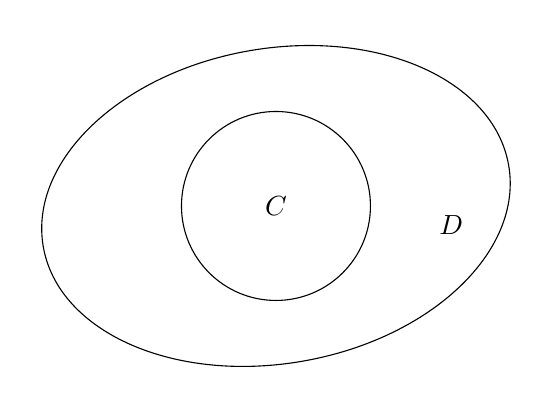
\begin{tikzpicture}
				\draw  (0,0) ellipse (1.2cm);
				\draw [rotate around={10:(0,0)}] (0,0) ellipse (3cm and 2cm);
				\draw (2.5,0) node[anchor=north east] {$D$};
				\draw (0,0) node {$C$};
			\end{tikzpicture} 
		\end{center}
		\caption{Diagrama de Venn de un conjunto $C$ incluido en un conjunto $D$.}
	\end{figure}
\end{center}

El conjunto vacío, que no tiene elementos, 
está incluido en \textbf{todos} los conjuntos, 
ya que ``todos'' sus elementos están en los demás conjuntos. 
Esto suena absurdo, y lo es, 
pero responde a la manera matemática de interpretar el cuantificador 
``para todo'', el cual puede cumplirse por ``vacuidad''.
Podemos decir, por ejemplo, que 
``todos los marcianos son verdes'' sin temor a errar 
ya que, al no existir marcianos, 
la afirmación no puede ser refutada, 
el conjunto de los marcianos es igual al conjunto vacío y, por lo tanto, 
está contenido en el conjunto de los elementos verdes.

En resumen, sea cual sea el conjunto $C$, se cumple que:
$$C\subseteq C\qquad \textrm{ y } \qquad \emptyset\subseteq C.$$

Algunas propiedades matemáticas pueden expresarse 
en forma de inclusión de conjuntos, veamos por ejemplo la afirmación:

\centerline{ Toda potencia natural de 3 es impar.}

La cual simbólicamente se puede escribir como:
$$\forall n\in \N\, ,\; 
\left(n\textrm{ es potencia de 3} \rightarrow n\textrm{ es impar}\right).$$
Si definimos los conjuntos:
\begin{eqnarray*} 
	A &=& \{3^n\ :\ n\in \N\}\\
	B &=& \{ m\in\N\ :\ m \textrm{ es impar}\}
\end{eqnarray*}

Resulta que lo afirmado más arriba equivale a decir $A\subseteq B.$

Así como un bicondicional es una conjunción de dos condicionales recíprocos, 
la igualdad de conjuntos es la conjunción de dos inclusiones recíprocas, 
tal como el siguiente lema expresa.

\medskip

\begin{lem}
	Dos conjuntos son iguales si y solo si cada uno está contenido en el otro.
\end{lem}

\medskip


El lema anterior se escribe de manera simbólica como sigue:
$$\forall\, C,D \textrm{ conjuntos}\,:\, C=D\ 
\Leftrightarrow\  
\left(C\subseteq D\wedge D\subseteq C\right).$$

Su demostración es directa de las definiciones de igualdad e inclusi\'on 
de conjuntos, en efecto:

{\em Dos conjuntos $C$ y $D$ son iguales si y solo si todo objeto que es elemento 
	de $C$ es elemento de $D$ y viceversa, es decir, 
	si y solo si $C$ está contenido en $D$ y viceversa.}

También podemos demostrarlo basándonos en lo que establecimos 
la semana pasada respecto a los conectivos lógicos, 
para esto asumimos que $C$ y $D$ son dos conjuntos cualesquiera, 
se tiene que:
\begin{eqnarray*}
	C=D &\Leftrightarrow& \forall x\,,\, 
	\left( x\in C \leftrightarrow x\in D\right)
	\qquad (\textrm{de la definición de igualdad})\\
	& \Leftrightarrow& \forall x \,,\,
	\left( x\in C \rightarrow x\in D\wedge x\in D \rightarrow x\in C\right)
	\qquad (\textrm{propiedad de bicondicional}),\\
	& \Leftrightarrow& \left(\forall x \,,\, 
	x\in C \rightarrow x\in D\right) \wedge 
	\left(\forall x\,,\, x\in D \rightarrow x\in C\right),\\
	& \Leftrightarrow&
	\left(C\subseteq D\right)\wedge \left(D\subseteq C\right) 
	\qquad (\textrm{de la definición de inclusión})
\end{eqnarray*}

Algunas propiedades matemáticas pueden expresarse 
en forma de inclusión o de igualdad 
de conjuntos. 

\medskip


\begin{ejemplo} 
	
Consideremos la afirmaci\'on\\

\centerline{Sea $a$ un n\'umero real.
	La ecuaci\'on $x^2+a=0$ tiene soluci\'on si y solo si $a \le 0$,}

la cual simbólicamente se puede escribir como:
$$\forall a\in \R\, ,\; 
\left(a\le 0\leftrightarrow \mbox{ la ecuaci\'on } x^2+a=0 \mbox{ tiene soluci\'on}\right).$$

Si definimos los conjuntos:
\[ 
	A = \{a \in \R\ :\ a \le 0\},\qquad 
	B = \{a \in \R\;:\;\mbox{la ecuaci\'on } x^2 + a = 0 \mbox{ tiene soluci\'on}\},
\]
resulta que lo afirmado más arriba equivale a decir $A = B$.
\end{ejemplo}

\medskip


\begin{ejemplo}
	La afirmaci\'on\\
	
	\centerline{Para todo n\'umero natural $n$ se cumple que si
	$n$ es m\'ultiplo de 6, entonces es par,}

	puede escribirse como inclusi\'on de dos conjuntos.
	Si definimos
	\[
		A = \{6n\;:\; n\in \N\},\qquad 
		B = \left\{2n\;:\; n\in \N\right\}
	\]
	la afirmaci\'on anterior es equivalente a $A \subseteq B$.
\end{ejemplo}

\medskip


\begin{ejemplo}\leavevmode
	Sean
	\[
		A = \{x\in \R\;:\; x^2 < 4\},\qquad 
		B = \left\{x \in \R\;:\; x < 2\right\}.
	\] 
	Demuestre que $A\subseteq B$, pero $A \ne B$.
	
	Los conjuntos $A$ y $B$ satisfacen
	$A \subseteq B$ si y solo si cualquier elemento
	de $A$ tambi\'en es elemento de $B$.
	Llamemos $y$ n\'umero real cualquiera.
	Debemos demostrar $y \in A \Rightarrow y \in B$.
	\[
		y \in A\;\Leftrightarrow \; 
		y^2 < 4 \; \Leftrightarrow\; |y| < 2\;\Leftrightarrow\;
		-2 < y < 2\; \Rightarrow \; y < 2 \; \Leftrightarrow\;
		y \in B.
	\]
	La l\'inea anterior es una demostraci\'on de $A \subseteq B$.
	Nota que partimos suponiendo que $y$ es un elemento cualquiera
	de $A$ y, haciendo uso de las definiciones de los conjuntos
	$A$ y $B$ y propiedades de los n\'umeros reales, obtuvimos 
	que $y \in B$.
	Al escribir el s\'imbolo $\Leftrightarrow$ entre dos argumentos
	de la demostraci\'on estamos indicando que ellos son equivalentes,
	por ejemplo, la desigualdad $y^2 < 4$ es equivalente a 
	$|y| < 2$. Nota, sin embargo, que no solo escribimos argumentos
	equivalentes, por ejemplo, $-2 < y < 2$ no es equivalente a 
	$y < 2$, sino solo podemos afirmar que si $-2 < y < 2$, entonces
	$y < 2$.
	
	Nos falta demostrar a\'un que, aunque $A \subseteq B$, los conjuntos
	$A$ y $B$ no son iguales, es decir, \textbf{hay} elementos de $B$ que no
	est\'an en $A$. ?`Notaste que escribimos en negritas 
	la palabra hay en la oraci\'on
	anterior? Lo hicimos para hacerte notar que solo nos falta
	encontrar un elemento de $B$ que no est\'e en $A$ para completar
	la demostraci\'on. Afortunadamente esto no es complicado pues
	ya sabemos que $A = \{z \in \R\;:\; -2 < z < 2\} = ]-2,\,2[$.
	Cualquier n\'umero real menor o igual que -2 es un ejemplo
	de un n\'umero real que es elemento de $B$ y no es elemento de $A$.
	Escribamos formalmente por qu\'e no es cierto que $B\subseteq A$,
	\[
		\left(-4 < 2 \;\Rightarrow\; -4 \in B\right)\,\wedge\,
		\left((-4)^2 = 16 \not < 4 \;\Rightarrow -4 \not \in A\right).
	\]
\end{ejemplo}

%\begin{ejemplo}
%	Demuestre que 
%	\[
%		\left\{3a + 7b\;:\; a,b\in \Z\right\} = \Z.
%	\]
%	
%	Debemos demostrar que dos conjuntos son iguales y sabemos que esto
%	es cierto si y solo si
%	\[
%		\left\{3a + 7b\;:\; a,b\in \Z\right\} \subseteq \Z\quad 
%		\wedge\quad 
%		\Z \subseteq \left\{3a + 7b\;:\; a,b\in \Z\right\}.
%	\]
%	
%	La primera de las inclusiones anteriores es sencilla pues si 
%	$a$ y $b$ son n\'umeros enteros, es cierto que $3a + 7b$ es un 
%	n\'umero entero.
%	
%	?`Qu\'e debemos hacer para demostrar la segunda inclusi\'on?
%	Debemos demostrar que cualquier n\'umero entero puede escribirse
%	en la forma $3a + 7b$. Entendamos mejor qu\'e significa esto, tomemos
%	algunos n\'umeros enteros:
%	\begin{align*}
%		0 = 3(0) + 7(0),\; 1 = 3(-2) + 7(1),\; 2 = 3(-4) + 7(2), \; 3 = 3(1) + 7(0),
%		\ldots
%	\end{align*}
%	
%	Si $x=0$, con $a=0$ y $b=0$, podemos escribir a $x$ en la forma $3a+7b$.
%	
%	Si $x=1$, con $a=-2$ y $b=1$, podemos escribir a $x$ en la forma $3a+7b$.
%	
%	?`Y si $x=-1$? Conociendo que $1 = 3(-2) + 7(1)$, 
%	sabemos que $-1 = 3(2) + 7(-1)$.
%	Solo debemos concentrarnos en encontrar los valores de $a$ y $b$ para
%	los n\'umeros naturales $x$, es decir, solo
%	debemos concentrarnos en demostrar
%	\[
%		\forall\,x\in \N\, ,\;\exists\,a,b \in \Z\, ,\; x = 3a+7b.
%	\]
%	
%	Sea $x$ un n\'umero natural cualquiera. Demostremos que existen $a$ y $b$ 
%	enteros de modo que $x = 3a+7b$.
%	Si $x$ es m\'ultiplo de 3, es sencillo determinar $a$ y $b$, ser\'ian 
%	$\frac x 3$ (es natural si $x$ es m\'ultiplo de 3) y $0$. 
%	
%	?`Qu\'e ocurre si $x$ no es m\'ultiplo de 3? Entonces $x$ es un n\'umero de
%	la forma $3m+1$ (el resto de $\frac x 3$ es 1), 
%	con $m\in \N$, o un n\'umero de la forma $3m+2$ (el resto de la divisi\'on
%	$\frac x 3$ es 2), pero 
%	\[
%		3m+1 = 3(m-2) + 7(1),\qquad 
%		3m+2 = 3(m-4) + 7(2),
%	\]
%	es decir, si $x$ es igual a $3m+1$ con $m\in \N$, entonces
%	con $a = m-2$ y $b=1$, $x$ puede escribirse como $3a+7b$, mientras
%	que si $x = 3m+2$, con $m\in \N$, entonces con $a=m-4$ y $b=2$, 
%	podemos escribir a $x$ como $3a+7b$.
%	
%	En resumen, si $x \in \Z$,
%	\[
%		\begin{cases}
%			\mbox{ si } x = 0 \; \Rightarrow a = 0,\; b = 0\\
%			\mbox{ si } x > 0 \; \Rightarrow
%		\begin{cases}
%			\mbox{si } x = 3m \mbox{ con  } m\in \N\;\Rightarrow & a = m,\; b =0,\\
%			\mbox{si } x = 3m+1 \mbox{ con  } m\in \N\;\Rightarrow & a=m-2,\; b=1,\\
%			\mbox{si } x = 3m+2 \mbox{ con  } m\in \N\;\Rightarrow & a=m-4,\; b=2.
%		\end{cases}
%		\end{cases}
%	\]
%	Por \'ultimo, si $x < 0$, determinamos $a$  y $b$ para $-x$.
%	Los inversos aditivos de estos valores son los correspondientes $a$ y $b$ 
%	para $-x$.
%	
%	Dado que hemos encontrado una forma de, para cualquier entero $x$,
%	determinar $a$ y $b$, de modo que $x=3a+7b$, hemos demostrado
%	que $\Z \subseteq \{3a + 7b\;:\; a,b \in \Z\}$ y esto, unido
%	a que $\{3a + 7b\;:\; a,b \in \Z\} \subseteq \Z$, garantiza
%	que $\Z= \{3a+7b\;:\;a,b\in \Z\}$.
%\end{ejemplo}


\section{Operaciones entre conjuntos}

Así como podemos operar números mediante las operaciones aritméticas, 
u operar proposiciones lógicas mediante los conectores lógicos, 
también podemos operar conjuntos.

\textbf{Unión:} La unión de dos conjuntos es el conjunto que 
reúne a los elementos de los dos conjuntos. 
Dicho de otra manera, si $C$ y $D$ son conjuntos, 
entonces su unión es un conjunto conformado por aquellos elementos 
que están en $C$ o en $D$, 
considerando al ``o'' de manera inclusiva, tal como 
dijimos la semana pasada.
El conjunto unión de $C$ con $D$ se denota por:
$$C\cup  D$$ y se lee ``{\em $C$ unión $D$}''.

\begin{center}
	\begin{figure}[h!]
		\begin{center}
			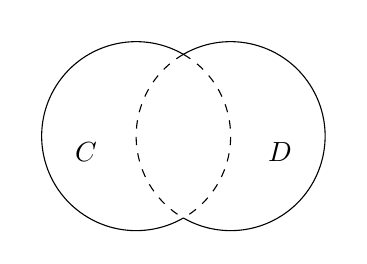
\begin{tikzpicture}
				\draw  (0,1) arc (60:300:1.2);
				\draw  (0,1) arc (120:-120:1.2);
				\draw[dashed]  (0,1) arc (60:-60:1.2);
				\draw[dashed]  (0,1) arc (120:240:1.2);
				\draw (1.5,0) node[anchor=north east] {$D$};
				\draw (-1.5,0) node[anchor=north west] {$C$};
			\end{tikzpicture} 
		\end{center}
		\caption{Diagrama de Venn de  $C$ unión $D$.}
	\end{figure}
\end{center}

Usando la definición de la unión: 
``{\em $C\cup D$ está conformado por aquellos elementos que 
	están en $C$ o en $D$}'', podemos describir el conjunto 
unión por comprensi\'on, valiéndonos del 
operador lógico ``{\em o}'', como sigue:
$$ C\cup  D=\{ x\\,:\, x\in C\vee x\in D\}.$$

De donde tenemos que:
$$\forall\, x\,:\, 
x\in C\cup  D\leftrightarrow x\in C\vee x\in D.$$

Esta definición resalta el carácter inclusivo del ``{\em o}'' matemático, 
ya que aquellos elementos que están en ambos conjuntos 
también forman parte de la unión.

\medskip


\begin{ejemplo}
	Veamos algunos ejemplos.
	\begin{itemize}
		\item $\{1,3,4,6\}\cup\{ 0,1,2\}=\{0,1,2,3,4,6\}$,
		\item $\{1,3,4,6\}\cup\emptyset = \{1,3,4,6\}$,
		\item $\{n\in\Z\ :\ n\textrm{ es par}\}
			\cup\{ n\in\Z\ :\ n\textrm{ es impar}\}=\Z$.
	\end{itemize}
\end{ejemplo}

\textbf{Intersección:} La intersección de dos conjuntos es 
el conjunto conformado por aquellos elementos que se 
encuentran en ambos conjuntos a la vez. Dicho de otra manera, 
si $C$ y $D$ son conjuntos, entonces su intersección 
está conformada por aquellos elementos que están en $C$ \textbf{y} 
en $D$.
El conjunto intersección de $C$ con $D$ se denota por:
$$ C\cap  D$$ y se lee ``{\em $C$ intersección $D$}''.

\begin{center}
	\begin{figure}[h!]
		\begin{center}
			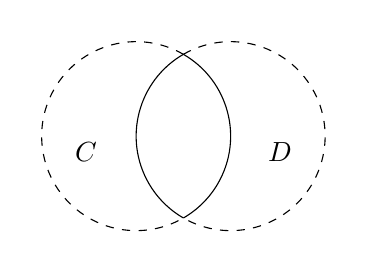
\begin{tikzpicture}
				\draw[dashed]  (0,1) arc (60:300:1.2);
				\draw[dashed]  (0,1) arc (120:-120:1.2);
				\draw  (0,1) arc (60:-60:1.2);
				\draw  (0,1) arc (120:240:1.2);
				\draw (1.5,0) node[anchor=north east] {$D$};
				\draw (-1.5,0) node[anchor=north west] {$C$};
			\end{tikzpicture} 
		\end{center}
		\caption{Diagrama de Venn de  $C$ intersección $D$.}
	\end{figure}
\end{center}

Usando la definición de la intersección: ``{\em $C\cap D$ 
	está conformado por aquellos elementos que están en $C$ y en $D$}'', 
podemos describir el conjunto intersección por comprensi\'on, 
valiéndonos del operador lógico ``{\em y}'', como sigue:

$$C\cap  D=\{ x\,:\,x\in C\wedge x\in D\}.$$

De donde tenemos que:

$$\forall\, x \,,\, 
x\in C\cap  D \leftrightarrow x\in C\wedge x\in D.$$

\begin{ejemplo}
	Algunos ejemplos.
	\begin{itemize}
		\item $\{1,3,4,6\}\cap\{ 0,1,2\}=\{1\}$,
		\item $\{1,3,4,6\}\cap\emptyset=\emptyset$,
		\item $\{n\in\Z\ :\ n\textrm{ es par}\}
			\cap\{ n\in\Z\ :\ n\textrm{ es impar}\}=\emptyset$,
		\item $\{n\in\N\ :\ n\textrm{ es par}\}\cap
			\{ n\in\Z\ :\ n\ge 4\}=\{ 2n\ :\ n\ge 2\}$.
	\end{itemize}
\end{ejemplo}


\textbf{Diferencia:} La diferencia $C\setminus D$  
es el conjunto conformado por aquellos elementos que pertenecen a $C$, 
pero no a $D$. 
El conjunto diferencia de $C$ menos $D$ se denota por:
$$ C\setminus  D.$$

\begin{center}
	\begin{figure}[h!]
		\begin{center}
			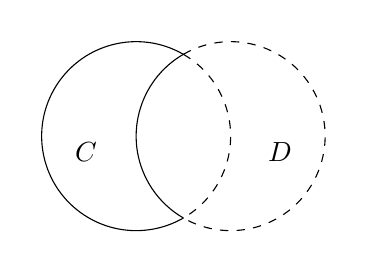
\begin{tikzpicture}
				\draw  (0,1) arc (60:300:1.2);
				\draw[dashed]  (0,1) arc (120:-120:1.2);
				\draw [dashed] (0,1) arc (60:-60:1.2);
				\draw  (0,1) arc (120:240:1.2);
				\draw (1.5,0) node[anchor=north east] {$D$};
				\draw (-1.5,0) node[anchor=north west] {$C$};
			\end{tikzpicture} 
		\end{center}
		\caption{Diagrama de Venn de  $C$ menos $D$.}
	\end{figure}
\end{center}

Usando la definición de la diferencia: 
``{\em $C\setminus D$ está conformado por aquellos elementos que 
	están en $C$ \textbf{ y no} en $D$}'', 
podemos describir el conjunto diferencia por comprensi\'on, 
valiéndonos del operador lógico ``{\em y}'' y la negación, como sigue:

$$C\setminus  D=\{ x \, : \,x\in C\wedge x\not\in D\}.$$

De donde tenemos que:
$$\forall\, x \,,\,
x\in C\setminus  D \leftrightarrow x\in C\wedge x\not\in D.$$

Se puede ver la diferencia de $C$ menos $D$ como el conjunto $C$ 
pero sacándole todo lo que haya de $D$ en él.

\textbf{Complemento:} Si el contexto permite definir un conjunto ``\emph{universo}'', $\mathcal{U}$ , por ejemplo en un problema que habla sobre naturales, el universo es $\N$, en uno que habla sobre reales, el universo es $\R$; es natural definir el ``\emph{complemento}'' de un conjunto. El complemento de un conjunto $C$ se denota $C^c$ y se define como:

$$C^c=\mathcal{U}\setminus C.$$

\medskip


\begin{ejemplo}
	Algunos ejemplos.
	\begin{itemize}
		\item $\{1,3,4,6\}\setminus\{0,1,2\}=\{3,4,6\}$,
		\item $\{ 0,1,2\}\setminus\{1,3,4,6\}=\{0,2\}$,
		\item $\{1,3,4,6\}\setminus\emptyset=
			\{1,3,4,6\}$,
		\item $\Z\setminus\{ n\in\Z\ :\ n\textrm{ es impar}\}=
			\{n\in\Z\ :\ n\textrm{ es par}\}$,
		\item $\{n\in\N\ :\ n\textrm{ es par}\}\setminus
			\{ n\in\Z\ :\ n\ge 4\}=\{ 0,2\}$.
		\item considerando $\mathcal{U}=\Z$, entonces $\{n\in\Z\ :\ n\textrm{ es par}\}^c=\{ n\in\Z\ :\ n\textrm{ es impar}\}$.
	\end{itemize}
\end{ejemplo}

Algunas propiedades que saltan a la vista son las siguientes.

\medskip


\begin{prop}
	Dados dos conjuntos cualesquiera $C$ y $D$
	se cumplen las siguientes afirmaciones:
	\begin{multicols}{2}
		\begin{itemize}
			\item $C\subseteq C\cup D$, 
			\item $D\subseteq C\cup D$,
			\item $C\cap D\subseteq C$,
			\item $C\cap D\subseteq D$,
			\item $C\setminus D\subseteq C$,
			\item Si $C\subseteq D$, entonces:
			\begin{itemize}
				\item $C\cup D=D$,
				\item $C\cap D=C$,
				\item $C\setminus D=\emptyset$,
				\item $D^c\subseteq C^c$.
			\end{itemize}
		\end{itemize}
	\end{multicols}
\end{prop}
\begin{ejemplo}\leavevmode
	Sean
	\[
	C = \left\{12x+3\;:\;x \in \Z\right\},\qquad 
	D = \left\{8x+2\;:\; x \in \Z\right\}.
	\]
	Demuestre que $C \cap D = \emptyset$.
	
	?`C\'omo podemos proceder para demostrar que $C \cap D = \emptyset$? 
	Nota que esto significa que debemos demostrar
	\[	
    \neg\exists\,x\in \Z\, ,\;x \in C\cap D\qquad
		\Leftrightarrow \qquad
		\forall\,x \in \Z \, ,\; \left[x\not \in C\,\vee \, x \not \in D\right],
	\]
	es decir, debemos demostrar que si $x$ es un n\'umero entero cualquiera,
	ocurre que $x$ no es elemento de $C$ o que $x$ no es elemento de $D$.
		
	Antes de comenzar a hacernos una idea de c\'omo podemos demostrar
	lo anterior debemos
	comprender qu\'e n\'umeros enteros pertenecen a cada conjunto.
	
	Si $x=0$, $12x+3 = 3$, por tanto $3 \in C$.
	Si $x=-1$, entonces $12x+3 = -9$ y si $x=1$, $12x+3 = 15$, los
	n\'umeros $-9$ y $15$ son elementos de $C$. Si seguimos asignando
	valores enteros a $x$ obtenemos 
	\[
	C = \{\ldots,-45, -33, -21, -9, 3, 15, 27, 39, 51, \ldots\}.
	\]
	\'Esta no pretende ser una definici\'on de $C$,
	con ella es dif\'icil comprender cu\'ales 
	n\'umeros enteros pertenecen al conjunto, solo la escribimos 
	para nombrar algunos elementos del conjunto.
	
	Si procedemos del mismo modo con $D$ tenemos que 
	\[
	D = \{\ldots,-30,-22,-14,-6,2,10,18,26,34,\ldots\}.		
	\]
	?`Notas alguna propiedad especial de los elementos de $C$ y $D$ que nos
	permita concluir que su intersecci\'on es el conjunto vac\'io?
	Observa que todos los elementos listados de $C$ son impares y todos los de 
	$D$ son pares. Si logramos demostrar que $C$ es un subconjunto del
	conjunto de los n\'umeros impares y que, por el contrario, $D$
	es subconjunto del conjunto de los n\'umeros pares, est\'a claro
	que su intersecci\'on es el conjunto vac\'io.
	
	Observa que si $x \in D$, entonces existe un n\'umero entero
	$m$ de modo que $x = 12m+3$, pero
	\[
	12m + 3 = 12m + 2 + 1 = 2(6m+1) + 1.
	\]
	Si $m\in \Z$, entonces $6m+1 \in \Z$ y, dado que hemos escrito
	a $x \in D$ en la forma $2k+1$ con $k\in \Z$, se cumple que 
	$x$ es impar.
	
	Por otro lado, si $x \in C$, entonces existe $m \in \Z$ de modo que
	$x = 8m + 2 = 2(4m+1)$. Si $m$ es un n\'umero entero,
	$4m+1$ tambi\'en lo es y, como hemos podido escribir a $x$ en la
	forma $2k$ con $k\in \Z$, se cumple que $x$ es par.
	
	As\'i, podemos concluir que si $x$ es un n\'umero entero cualquiera,
	$x$ es par o impar. Si es par, entonces no pertenece a $C$ y si es impar,
	no pertenece a $D$, esto significa que $C \cap D = \emptyset$.
\end{ejemplo}

Igualmente, los conjuntos heredan algunas de las propiedades de la lógica.

\begin{prop}
Dados $A$, $B$, $C$ conjuntos, se cumplen las siguientes igualdades.
\begin{itemize}

% mod lbh 24.2.05
%%%%%%%%%%%%%%%%%%%
\item %$ A \cup A = A\quad  \land \quad A\cap A = A $\quad
$ A \cup A = A\:, \quad A\cap A = A $\quad
(idempotencia)

\item %$ A \cup B = B\cup A \quad \land \quad A\cap B = B \cap A$ \quad
$ A \cup B = B\cup A\:, \quad A\cap B = B \cap A$ \quad
(conmutatividad de $ \cup$ y $ \cap$)

\item $ A\cup (B\cup C) = (A\cup B) \cup C$ \quad (asociatividad de $ \cup$)

\item
$ A \cap (B\cap C) = (A\cap B) \cap C$ \quad (asociatividad de $ \cap$)

\item $ A\cup(B\cap C) = (A\cup B) \cap (A\cup C)$ 
(distributividad de $ \cup$ con respecto a $ \cap$)

\item
$ A\cap (B\cup C) = (A\cap B) \cup (A\cap C)$ 
(distributividad de $ \cap$ con respecto a $ \cup$)

\item
$ (A\cup B)^c\,=\,A^c \cap B^c$ \quad (Ley de De Morgan)

\item
$ (A\cap B)^c\,=\,A^c \cup B^c$ \quad (Ley de De Morgan)

\end{itemize}
\end{prop}

\medskip

Finalmente, introducimos una definición que se usa bastante y habla de cuando los conjuntos no tienen ningún elemento en común.

\medskip

\begin{defn}
Dos conjuntos $ A$ y $ B$ se dicen {disjuntos} si y s\'olo si
$ A \cap B = \phi$.
\end{defn}

\medskip

Siempre se cumple que $C$ es disjunto a $C^c$, $D$ es disjunto a $C\setminus D$, y $\emptyset$ es disjunto a todo conjunto (incluso a sí mismo).

\section{Conjunto potencia}

El {\em conjunto  potencia} de un conjunto $C$ es 
un conjunto cuyos elementos son todos los subconjuntos posibles de  
$C$, incluyendo a $C$ mismo y al conjunto vacío.
El conjunto potencia se denota por:

$$\mathcal{P}(C).$$

Usando su definición, podemos describir 
el conjunto intersección por notación intensiva, como sigue:
\[\mathcal{P}(C)=\{A: A\subseteq C\}.\]

De donde tenemos que:

$$A\in \mathcal{P}(C) \Leftrightarrow A\subseteq C.$$

Es algo complejo imaginar un conjunto de conjuntos, 
es decir un conjunto cuyos elementos son conjuntos.

Un ejemplo simple podría ser:  $B=\{ \{1,2\},\{1,3,5\},\emptyset\}$. 
Vemos que $B$ tiene 3 elementos (son los 3 objetos que están entre la primera 
llave de apertura y la última llave de cierre, 
separados por las dos comas ``,'').
Cada uno de sus elementos es un conjunto: 
$\{1,2\}$ es uno de sus elementos, $\{1,3,5\}$ es otro y $\emptyset$ es otro.
Los 3 son conjuntos.

Los elementos del conjunto potencia de $C$ 
son conjuntos, pero no son cualquier conjunto, sino
aquellos que son subconjuntos de $C$. 
Por ejemplo, tenemos que:

$$\mathcal{P}(\{3,5\})=  \{ \emptyset, \{3\},\{5\},\{3,5\}\},$$

$$\mathcal{P}(\{1,2,3\})=  \{\emptyset,
\{1\},\{2\},\{3\},\{1,2\},\{1,3\},
\{2,3\},\{1,2,3\}\}.$$

Es algo mareador leer estos conjuntos, pero las llaves están para ayudar, 
lo primero que hay que hacer es emparejar 
las llaves consecutivas opuestas entre sí, 
usaremos colores para facilitar la tarea,

$$\mathcal{P}(\{1,2,3\})=  \{\emptyset, \color{red}{\{1\}}\color{black},
\color{orange}{\{2\}}\color{black},
\color{green}{\{3\}}\color{black},
\color{cyan}{\{1,2\}}\color{black},
\color{blue}{\{1,3\}}\color{black},
\color{violet}{\{2,3\}}\color{black},
\color{magenta}{\{1,2,3\}}\color{black}{\}}.$$

Estas llaves coloreadas encierran a los conjuntos 
cuyos elementos no son conjuntos, \'estos son todos 
subconjuntos de $\{1,2,3\}$, 
de hecho son todos los subconjuntos de $\{1,2,3\}$; 
y \'estos son los 8 elementos del conjunto de las partes de 
$\{1,2,3\}$, el cual se lee partiendo desde la primera 
llave de apertura (en negro), y terminando en la siguiente 
llave de cierre que no esté 
ya emparejada con otra llave de apertura.

Un caso delicado e interesante de analizar es el conjunto 
de las partes del conjunto vacío. 
Por supuesto \'este no es vacío, 
ya que el vacío es subconjunto de todos los conjuntos, 
en particular es subconjunto de sí mismo, 
de manera que el vacío es un elemento del conjunto de las partes del vacío:

$$\mathcal{P}(\emptyset)=  \{ \emptyset \}.$$

Así, $\emptyset$ tiene 0 elementos, 
mientras que $\mathcal{P}(\emptyset)=  \{ \emptyset \}$ 
tiene un elemento, no es vacío, 
pues contiene al conjunto vacío: $\emptyset\not = \{ \emptyset\}$.

\textbf{ Propiedades}.
\begin{enumerate}
\item $A\subseteq B \Rightarrow \mathcal{P}(A)\subseteq \mathcal{P}(B)$.
\item $\mathcal{P}(A)\subseteq \mathcal{P}(B) \Rightarrow A\subseteq B$.
\item $\mathcal{P}(A)= \mathcal{P}(B) \Leftrightarrow A= B$.
\end{enumerate}
\textbf{ Dem.}

1) p.d.q. $C\subseteq A \Rightarrow C\subseteq B$, en efecto, 
si $C\subseteq A$ y $A\subseteq B$ entonces $C\subseteq B$. $\Box$

2) {\em (versi\'on incorrecta) Si $\mathcal{P}(A)\subseteq \mathcal{P}(B)$, 
	entonces todo conjunto de $\mathcal{P}(A)$ est\'a contenido en todo 
	conjunto de $\mathcal{P}(B)$, y como $A\in \mathcal{P}(A)$ y $B\in \mathcal{P}(B)$,  
	$A\subseteq B$.}

2) p.d.q. $A\subseteq B$, en efecto, $A\in \mathcal{P}(A)$ y $\mathcal{P}(A)\subseteq \mathcal{P}(B)$, 
de donde $A\in \mathcal{P}(B)$, lo que significa que $A\subseteq B$.$\Box$

3) $A=B$ trivialmente implica que $\mathcal{P}(A)= \mathcal{P}(B)$. Por otra parte,
Si $\mathcal{P}(A)= \mathcal{P}(B)$, entonces $\mathcal{P}(A)\subseteq \mathcal{P}(B)$ y 
$\mathcal{P}(A)\subseteq \mathcal{P}(B)$, y por 2) esto implica que $A\subseteq B$ y 
$B\subseteq A$.$\Box$

\textbf{ Ejercicios:}
Considere $A\subseteq U$.\\ 
>Qu\'e puede decir de $\mathcal{P}(U-A)$ con respecto a $\mathcal{P}(U)-\mathcal{P}(A)$?\\
>Qu\'e puede decir de $\mathcal{P}(A\cap B)$ c/r a $\mathcal{P}(A)\cap \mathcal{P}(B)$?\\
>Qu\'e puede decir de $\mathcal{P}(A\cup B)$ c/r a $\mathcal{P}(A)\cup \mathcal{P}(B)$?\\



\section{Cardinalidad de conjuntos finitos}

Lo primero que aprendimos en la enseñanza básica fue a contar, en esa época, todos esos conjuntos eran conjuntos \emph{finitos}, partíamos contando, y el algún momento terminábamos de contar, entonces sabíamos qué cantidad de elementos tenía el conjunto.
Hoy,  tal número lo llamamos formalmente el \emph{cardinal} del conjunto.
Si $A$ es un conjunto finito, su cardinal lo denotamos por $|A|$ y es un número natural,  o bien 0, si es que $A=\emptyset$.

A los conjuntos \emph{infinitos} también se les puede asociar un cardinal, pero eso excede los contenidos de este curso y es más bien de interés de la matemática pura y otras disciplinas abstractas.


\medskip

\begin{defn}
La {\em cardinalidad de un conjunto finito} $A$, se representa $|A|$, es el n\'umero de elementos de $A$.
\end{defn}


\medskip

\begin{ejemplo}\leavevmode 
	
	$|\emptyset| = 0$, 	
	$\left|\left\{\emptyset\right\}\right| = 1$, 
	
	?`Entiendes que
	$\{\emptyset\}$ y $\emptyset$ no son lo mismo? El primero es el conjunto
	cuyo \'unico elemento es el conjunto vac\'io, mientras el segundo es
	el conjunto vac\'io, el que no tiene elementos. 
	
	?`Cu\'al es la cardinalidad
	de $\{\emptyset, \{\emptyset\}, \{\emptyset, \{\emptyset\}\}\}$?
	Identifica primero cu\'ales son sus elementos.
	
	$|\{1,2\}| = 2$, $|\{2,3\}| = 2$.
	
	Nota que $|\{1,2\}\cup\{2,3\}| = |\{1,2,3\}| = 3 = 
	|\{1,2\}| + |\{2,3\}| - |\{1,2\}\cap \{2,3\}|$.
\end{ejemplo}

El cardinal de un conjunto es un atributo de gran importancia, nos sirve mucho en probabilidaes, pero también en planificaición, manejo de inventario, combinatoria, etc.
Sus propiedades en relación a las demás operaciones y relaciones de conjuntos es de gran relevancia.

\begin{prop}
Dados dos conjuntos finitos $A$ y $B$, se cumple:
\begin{itemize}
\item Si $A\subseteq B$, entonces $|A|\le |B|$,
\item $|\mathcal{P}(A)|=2^{|A|}$,
\item $|\emptyset|=0$.
\item Si $A$ y $B$ son disjuntos, entonces $|A\cup B|=|A|+|B|$.
\end{itemize}
\end{prop}

Pero la propiedad más interesante es qué pasa con $|A\cup B|$ cuando $A$ y $B$ no son disjuntos, para ver esto, podemos descomponer $A\cup B$ en partes disjuntas. 
Usando la operación de diferencia, no es difícil ver que
\[ A\cup B=(A\setminus B)\cup (A\cap B)\cup (B\setminus A)\]
Donde $A\setminus B$, $A\cap B$ y $B\setminus A$ son todos disjuntos unos con otros.

Notamos que tenemos:
\[A=(A\setminus B)\cup (A\cap B)\quad \textrm{ y } \quad B=(A\cap B)\cup (B\setminus A)\]
y como se trata de la unión de conjuntos disjuntos, se tiene que
\[|A|=|A\setminus B|+ |A\cap B|\quad  \textrm{ y } \quad |B|=|A\cap B| + |B\setminus A|.\]

Por lo tanto podemos obtener la siguiente fórmula:

\[|A\cup B|=|A|+|B|-|A\cap B|\]

Otra forma de explicarla es notar que si simplemente sumamos $|A|$ con $|B|$, estamos contando dos veces los elementos de $A\cap B$, por lo cual debemos restarlos.

Trabajando un poco más, se obtiene la siguiente fórmula para 3 conjuntos.

\begin{prop}
Si $ A$, $ B$ y $ C$ son conjuntos arbitrarios, entonces
$$ |A\cup B\cup C|\,=\,|A|+|B|+|C|-|A\cap B|-|A\cap C|-|B\cap C| + |A\cap B\cap C|\,.$$
\end{prop}
\begin{proof}
\begin{align*}
	|A\cup (B \cup C)| &= |A| + |B\cup C| - |A \cap (B\cup C)|,\\
	&= |A| + |B| + |C| - |B \cap C| - |(A \cap B) \cup (A \cap C)|,\\
	&= |A| + |B| + |C| - |B \cap C| - |A \cap B| - |A \cap C| + |A \cap B \cap C|
\end{align*}
\end{proof}

\begin{ejercicio} 
Mediante operaciones de conjuntos, describa todos los conjuntos disjuntos que aparecen el el siguiente diagrama de Venn.

\begin{center}
	\begin{figure}[h!]
		\begin{center}
			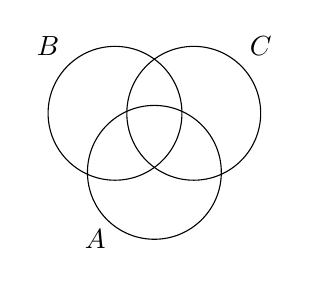
\begin{tikzpicture}[scale=0.5]
				\draw  (0,0) circle (1.7cm);
				\draw  (1,1.5) circle (1.7cm);
				\draw  (-1,1.5) circle (1.7cm);
				\draw (-1.5,-1.7) node {$A$};
				\draw (-2.7,3.2) node {$B$};
				\draw (2.7,3.2) node {$C$};
			\end{tikzpicture} 
		\end{center}
		\caption{Diagrama de Venn de 3 conjuntos arbitrarios.}
	\end{figure}
\end{center}
\end{ejercicio}

\medskip

Veamos un par de ejemplos donde puedes utilizar las propiedades anteriores.
Seguramente ya has resuelto problemas como \'estos durante la ense\~nanza
media.



\begin{ejemplo}\label{eje:i1}
	De una encuesta realizada a un grupo de 55 personas que han recibido
	cursos avanzados de ingl\'es, franc\'es y/o alem\'an, se sabe que
	45 de ellas han recibido cursos avanzados de ingl\'es, 32 de 
	franc\'es, 22 de alem\'an y 10 de los tres idiomas. 
	?`Cu\'antas de estas personas
	han recibido cursos avanzados de exactamente 2 idiomas?\\
	
	\begin{center}
	\begin{figure}[h!]
		\begin{center}
			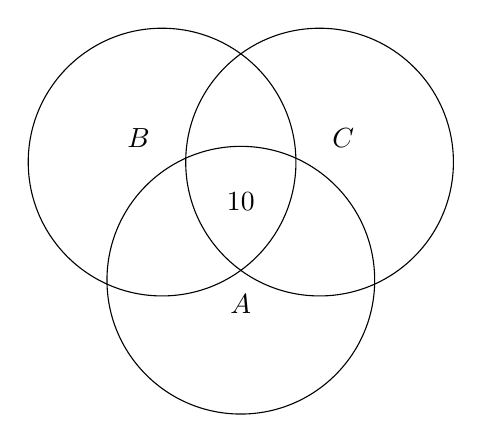
\begin{tikzpicture}
				\draw  (0,0) circle (1.7cm);
				\draw  (1,1.5) circle (1.7cm);
				\draw  (-1,1.5) circle (1.7cm);
				\draw (0,-0.3) node {$A$};
				\draw (-1.3,1.8) node {$B$};
				\draw (1.3,1.8) node {$C$};
				\draw (0,1) node {$10$};
			\end{tikzpicture} 
		\end{center}
		\caption{Ejemplo~\ref{eje:i1}}
	\end{figure}
\end{center}
	
	Si $A$ es el conjunto de personas que han recibido cursos avanzados de ingl\'es,
	$B$ el de las que ha recibido cursos avanzados de franc\'es y
	$C$ el de las que los ha recibido de alem\'an, entonces
	\[
		|{\mathcal U}| = |A\cup B\cup C| = 55, |A| = 45, |B| = 32, |C| = 22,
		|A\cap B\cap C| = 10.
	\]
	Se tiene entonces que
	\begin{align*}
		|A\cup B \cup C| &= 55 = |A| + |B| + |C| - 
		(|A\cap B| + |A\cap C| + |B\cap C|) + 	|A\cap B\cap C|,\\
		&= 99 - (|A\cap B| + |A\cap C| + |B\cap C|) + 10.
	\end{align*}
	Por tanto,
	\[
		|A\cap B| + |A\cap C| + |B\cap C| = 54.
	\]
	La cantidad de personas que han cursado exactamente dos idiomas
	no es $|A\cap B| + |A\cap C| + |B\cap C|$, sino 
	$|A\cap B| + |A\cap C| + |B\cap C| - 3|A\cap B\cap C| = 24$, 
	al sumar las cardinalidades 
	de $A\cap B$, $A\cap C$ y $B\cap C$ se suma 3 veces 
	$|A\cap B\cap C|$, pero solo nos interesa conocer cu\'antas
	personas han cursado exactamente dos idiomas, no los tres.			
\end{ejemplo}

\begin{ejemplo}\label{eje:i2}
	En un liceo hay 1186 estudiantes, de los cuales 879 hacen un curso intensivo de ingl\'es, 378 uno
	de alem\'an y 690 uno de franc\'es. 
	Si sabemos que 506 estudiantes estudian ingl\'es y franc\'es,
	77 alem\'an y franc\'es, 13 los tres idiomas y 159, 
	estudian alem\'an, pero no ingl\'es, averig\"ue
	cu\'antos estudiantes no estudian ning\'un idioma y 
	cu\'antos estudian s\'olo ingl\'es y alem\'an.
	
		\begin{center}
	\begin{figure}[h!]
		\begin{center}
			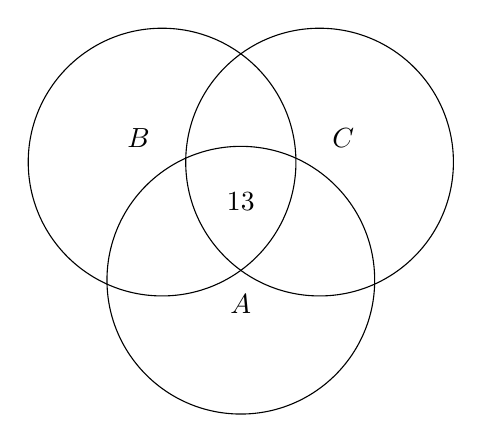
\begin{tikzpicture}
				\draw  (0,0) circle (1.7cm);
				\draw  (1,1.5) circle (1.7cm);
				\draw  (-1,1.5) circle (1.7cm);
				\draw (0,-0.3) node {$A$};
				\draw (-1.3,1.8) node {$B$};
				\draw (1.3,1.8) node {$C$};
				\draw (0,1) node {$13$};
			\end{tikzpicture} 
		\end{center}
		\caption{Ejemplo~\ref{eje:i2}}
	\end{figure}
\end{center}

	
	Si $A$ denota al conjunto de estudiantes que estudian alem\'an, 
	$I$ al de los que estudian ingl\'es
	y $F$ al de los que estudian franc\'es, entonces sabemos que 
	\[
	|I| = 879,\quad |A| = 378,\quad |F| = 690.
	\]
	Adem\'as 
	\[
	|I \cap F| = 506,\quad |F \cap A| = 77,\quad |I \cap A \cap F| = 13, 
	\quad |A\setminus I| = 159.
	\]
	Nos piden determinar cu\'antos no estudian ning\'un idioma. 
	El n\'umero de estudiantes que no estudia ning\'un idioma 
	es igual al n\'umero total de estudiantes
	menos la cantidad de estudiantes que estudia al menos un idioma, la cual es la cardinalidad
	del conjunto $A \cup I \cup F$.
	
	Sabemos que 
	\begin{align*}
		|A \cup F \cup I| &= |A| + |I| + |F| - 
		|A \cap F| - |A \cap I| - |I \cap F| + |A \cap I \cap F|,\\
		&= 378 + 879 + 690 - 77 - |A \cap I| - 506 + 13 = 1377 - |A \cap I|.
	\end{align*}
	?`C\'omo determinar $|A \cap I|$? Conocemos $|A \setminus I|$, $|A|$, $|I|$. 
	Pero $A = (A\setminus I) \cup (A \cap I)$ (un estudiante
	toma curso de alem\'an si y solo si toma alem\'an y no toma ingl\'es, pertenece
	a $A \setminus I$, o toma tanto alem\'an como ingl\'es, pertenece a 
	$A \cap I$).

	Entonces $|A| = |A\setminus I| + |A \cap I| - |(A\setminus I)\cap (A\cap I)| = 
	|A\setminus I| + |A \cap I| - |\emptyset|$.
	Por tanto, $|A \cap I| = 378 - 159 = 219$ y
	$|A \cup F \cup I| = 1158$ y 
	la cantidad de estudiantes que no estudia ning\'un
	idioma es $1186 - |A\cup I\cup F| = 1186-1158 = 28$.
	
	Tambi\'en debemos determinar la cantidad de estudiantes 
	que estudian s\'olo ingl\'es
	y alem\'an. Si llamamos 
	$IA$ a este nuevo conjunto, 
	${\mathcal S }= (I \cap A)\setminus (I\cap A \cap F)$ 
	y se tiene que 
	\[
		I\cap A = {\mathcal S} \cup (I\cap A \cap F),\qquad 
		{\mathcal S} \cap (I\cap A \cap F) = \emptyset.
	\]
	Con esto tenemos que 
	$|I\cap A| = |{\mathcal S}| + |I \cap A \cap F|$
	y $|{\mathcal S}| = |I\cap A| - |I \cap A \cap F|
	= 219 - 13 = 206$.			
\end{ejemplo}

